% 16:9 LaTeX/TikZ presentation. Build with make from this directory.
% Editable source for PGConf.EU Valencia, 20 October 2026.
% All historical SQL is labelled. Contemporary examples use TAS-028R1 syntax.
% Current presenter notes and provenance are kept beside each slide below.
% Earlier Markdown presenter guides are preserved in archive/.
\documentclass[12pt]{article}
\usepackage[paperwidth=400mm,paperheight=225mm,margin=0mm]{geometry}
\usepackage[T1]{fontenc}
\usepackage{lmodern}
\renewcommand{\familydefault}{\sfdefault}
\usepackage{tikz}
\usepackage{listings}
\usetikzlibrary{calc,arrows.meta}
\usepackage[pdfauthor={Andreas Karlsson and Joel Jacobson},
pdftitle={Designing a new SQL language feature: Key joins},
pdfsubject={PGConf.EU 2026, Valencia},hidelinks]{hyperref}
\pagestyle{empty}
\setlength{\parindent}{0pt}
\hyphenpenalty=10000
\exhyphenpenalty=10000
\definecolor{ink}{HTML}{192B3A}
\definecolor{muted}{HTML}{52616D}
\definecolor{blue}{HTML}{205C8D}
\definecolor{teal}{HTML}{176B60}
\definecolor{orange}{HTML}{A34727}
\definecolor{rulecolor}{HTML}{CCD5DB}
\definecolor{pale}{HTML}{F0F5F8}
\newcommand{\txt}[7]{\node[anchor=north west,inner sep=0pt,align=left,
text width=#3mm,text=#6,font=\fontsize{#4}{#5}\selectfont] at (#1,#2) {#7};}
\newcommand{\codeat}[5]{\node[anchor=north west,inner sep=0pt,text=ink,
font=\ttfamily\fontsize{#3}{#4}\selectfont] at (#1,#2)
{\begin{tabular}{@{}l@{}}#5\end{tabular}};}
% Stable calendar scale: 1 January 2021 through 31 December 2026.
% Marker positions are truncated to the first day of their calendar month.
% Same-month events/ranges use one large dot; multi-month ranges use a segment.
% The subtitle gives date precision. Approximate intervals are labelled as such.
% Proposal labels identify meeting stages, not paper-cover or invention dates.
% Gregorian day offsets for this fixed 2021--2026 window, with no extra package.
\def\TimelineMonthStart#1{\ifcase#1\or0\or31\or59\or90\or120\or151\or181\or212\or243\or273\or304\or334\fi}
\def\TimelineSplitDate#1-#2-#3\relax#4{%
  \edef\TimelineMonth{\number\numexpr#2\relax}%
  \def\TimelineDay{1}% Month precision; retain the original dates in slide metadata.
  \pgfmathtruncatemacro{\TimelineLeapDay}{and(mod(#1,4)==0,\TimelineMonth>2)}%
  \pgfmathsetmacro{#4}{20+((365*(#1-2021)+floor((#1-2021)/4)+\TimelineMonthStart{\TimelineMonth}+\TimelineDay-1+\TimelineLeapDay)/2190)*360}%
}
\newcommand{\TimelineDateX}[2]{%
  \edef\TimelineExpandedDate{#1}%
  \expandafter\TimelineSplitDate\TimelineExpandedDate\relax{#2}%
}
\newcommand{\TimelineFocus}[4]{%
  \def\TimelineMode{#1}% 0 no cursor, 1 event, 2 period
  \def\TimelineStartDate{#2}%
  \def\TimelineFinishDate{#3}%
  \def\TimelineActiveProposal{#4}%
}
\newcommand{\TimelineRegister}[5]{%
  \expandafter\def\csname TimelineSlide#1\endcsname{\TimelineFocus{#2}{#3}{#4}{#5}}%
}
% Per-slide chronology. Empty dates mean that a historical cursor is not useful.
\TimelineRegister{1}{0}{}{}{}
\TimelineRegister{2}{0}{}{}{}
\TimelineRegister{3}{2}{2021-03-27}{2026-10-12}{}
\TimelineRegister{4}{0}{}{}{}
\TimelineRegister{5}{0}{}{}{}
\TimelineRegister{6}{1}{2021-03-27}{2021-03-27}{}
\TimelineRegister{7}{2}{2021-03-27}{2021-03-31}{}
\TimelineRegister{8}{2}{2021-03-28}{2021-03-31}{}
\TimelineRegister{9}{2}{2021-03-28}{2022-05-09}{}
\TimelineRegister{10}{2}{2021-12-01}{2022-03-31}{}
\TimelineRegister{11}{2}{2022-01-24}{2022-05-09}{}
\TimelineRegister{12}{2}{2022-05-09}{2023-09-27}{CMN-023}
\TimelineRegister{13}{2}{2023-09-28}{2024-09-30}{}
\TimelineRegister{14}{2}{2024-09-30}{2024-10-25}{}
\TimelineRegister{15}{1}{2024-10-06}{2024-10-06}{}
\TimelineRegister{16}{1}{2024-10-23}{2024-10-23}{}
\TimelineRegister{17}{1}{2025-02-08}{2025-02-08}{}
\TimelineRegister{18}{2}{2024-12-21}{2025-07-17}{POS-009}
\TimelineRegister{19}{2}{2025-09-22}{2025-12-08}{BCN-060}
\TimelineRegister{20}{2}{2025-10-21}{2025-10-24}{}
\TimelineRegister{21}{2}{2025-12-09}{2025-12-11}{W30-020}
\TimelineRegister{22}{2}{2025-12-08}{2025-12-11}{W30-020}
\TimelineRegister{23}{2}{2026-03-12}{2026-05-28}{}
\TimelineRegister{24}{2}{2026-04-02}{2026-04-21}{}
\TimelineRegister{25}{1}{2026-04-04}{2026-04-04}{}
\TimelineRegister{26}{1}{2026-04-21}{2026-04-21}{}
\TimelineRegister{27}{1}{2026-05-28}{2026-05-28}{}
\TimelineRegister{28}{2}{2026-06-15}{2026-06-19}{BMA-015}
\TimelineRegister{29}{2}{2026-06-15}{2026-09-30}{W32-024}
\TimelineRegister{30}{2}{2026-08-18}{2026-09-20}{TAS-028}
\TimelineRegister{31}{1}{2026-10-12}{2026-10-12}{TAS-028}

\TimelineRegister{32}{0}{}{}{}
\TimelineRegister{33}{0}{}{}{}
\TimelineRegister{34}{0}{}{}{}



\TimelineRegister{35}{0}{}{}{}

\newcommand{\TimelineProposal}[4]{%
  \TimelineDateX{#1}{\TimelineProposalX}%
  \def\TimelineProposalCode{#2}%
  \ifx\TimelineProposalCode\TimelineActiveProposal
    \def\TimelineProposalColor{blue}%
    \def\TimelineProposalWeight{\bfseries}%
  \else
    \def\TimelineProposalColor{muted}%
    \def\TimelineProposalWeight{}%
  \fi
  \draw[\TimelineProposalColor!55,line width=.45pt]
    (\TimelineProposalX,13.5) -- (#3,#4-1.2);
  \fill[\TimelineProposalColor] (\TimelineProposalX,12.5) circle[radius=.65mm];
  \node[anchor=north,inner sep=0pt,text=\TimelineProposalColor,
    font=\fontsize{10.5}{12.6}\selectfont\TimelineProposalWeight] at (#3,#4) {#2};
}
% Conference milestones above the axis; WG3 proposal labels remain below it.
% Dates: Athens 22--25 October 2024; Riga 21--24 October 2025;
% Vancouver 19--22 May 2026. Marker placement uses the shared month precision.
\newcommand{\TimelineConference}[3]{%
  \TimelineDateX{#1}{\TimelineConferenceX}%
  \draw[teal!65,line width=.45pt]
    (\TimelineConferenceX,11.6) -- (\TimelineConferenceX,10);
  \draw[teal,line width=.65pt,fill=white]
    (\TimelineConferenceX-.65,11.85) rectangle (\TimelineConferenceX+.65,13.15);
  \node[anchor=south,inner sep=0pt,align=center,text=teal,
    font=\fontsize{10}{11.5}\selectfont] at (\TimelineConferenceX,9.3) {#2\\#3};
}
\newcommand{\timeline}[1]{%
  \csname TimelineSlide#1\endcsname
  \draw[rulecolor,line width=1pt] (20,12.5) -- (380,12.5);
  \ifnum\TimelineMode>0
    \TimelineDateX{\TimelineStartDate}{\TimelineStartX}%
    \TimelineDateX{\TimelineFinishDate}{\TimelineFinishX}%
    % An interval needs at least two distinct months; otherwise use one dot.
    \ifnum\TimelineMode=2
      \ifdim\TimelineStartX pt=\TimelineFinishX pt
        \def\TimelineMode{1}%
      \fi
    \fi
    \draw[blue!35,line width=1.3pt] (20,12.5) -- (\TimelineStartX,12.5);
    \ifnum\TimelineMode=2
      \draw[blue!13,line width=5mm,line cap=round]
        (\TimelineStartX,12.5) -- (\TimelineFinishX,12.5);
      \draw[blue,line width=2.6pt]
        (\TimelineStartX,12.5) -- (\TimelineFinishX,12.5);
    \fi
  \fi
  \foreach \yr in {2021,...,2026}{%
    \TimelineDateX{\yr-01-01}{\TimelineYearX}%
    \draw[rulecolor,line width=.6pt] (\TimelineYearX,10.6) -- (\TimelineYearX,14.4);
    \node[text=muted,inner sep=0pt,font=\fontsize{12}{14.4}\selectfont]
      at (\TimelineYearX,5) {\yr};
  }
  \TimelineConference{2024-10-22}{PGConf.EU}{Athens 2024}
  \TimelineConference{2025-10-21}{PGConf.EU}{Riga 2025}
  \TimelineConference{2026-05-19}{PGConf.dev}{Vancouver 2026}
  % Lower label row separates W30/W32 from their neighbouring proposal stages.
  % UTC/CMN dates are scheduled presentation days corroborated by meeting minutes;
  % other stages use meeting starts where the discussion day is not established.
  \TimelineProposal{2023-02-10}{UTC-107}{146.67}{17.2}
  \TimelineProposal{2023-09-27}{CMN-023}{184.49}{17.2}
  \TimelineProposal{2025-03-10}{POS-009}{271.3}{17.2}
  \TimelineProposal{2025-09-22}{BCN-060}{303.5}{17.2}
  \TimelineProposal{2025-12-09}{W30-020}{316.4}{22.2}
  \TimelineProposal{2026-06-15}{BMA-015}{347.4}{17.2}
  \TimelineProposal{2026-08-18}{W32-024}{358}{22.2}
  \TimelineProposal{2026-10-12}{TAS-028}{367.2}{17.2}
  % Draw the focus last so its white outline stays visible over milestone dots.
  \ifnum\TimelineMode=1
    \filldraw[fill=blue,draw=white,line width=.7mm]
      (\TimelineStartX,12.5) circle[radius=2.35mm];
  \fi
  \ifnum\TimelineMode=2
    \filldraw[fill=blue,draw=white,line width=.4mm]
      (\TimelineStartX,12.5) circle[radius=1.1mm];
    \filldraw[fill=blue,draw=white,line width=.4mm]
      (\TimelineFinishX,12.5) circle[radius=1.1mm];
  \fi
}
\newenvironment{slide}[5]{%
\clearpage\null
\begin{tikzpicture}[remember picture,overlay,x=1mm,y=-1mm]
\begin{scope}[shift={(current page.north west)}]
\timeline{#1}
\txt{18}{28}{365}{14}{17}{blue}{#2}
\txt{18}{42}{365}{32}{38}{ink}{\textbf{#3}}
\draw[rulecolor,line width=.5pt] (18,210) -- (382,210);
\txt{18}{215}{340}{10.5}{12.6}{muted}{#4}
\node[anchor=north east,inner sep=0pt,text=muted,font=\fontsize{11}{13}\selectfont] at (382,215) {#5};
}{\end{scope}\end{tikzpicture}}

% The opening fanout example uses fixed-pitch SQL, ASCII results and diagnostics.
% These styles are local to its listings; the rest of the deck is unchanged.
\lstdefinestyle{fanout-mono}{
  language={},
  basicstyle=\ttfamily\fontsize{12}{16}\selectfont\color{ink},
  keywordstyle={},identifierstyle={},commentstyle={},stringstyle={},
  columns=fixed,basewidth=.525em,keepspaces=true,tabsize=4,
  showstringspaces=false,showspaces=false,showtabs=false,
  breaklines=false,numbers=none,frame=none,upquote=true,
  aboveskip=0pt,belowskip=0pt,
  xleftmargin=0pt,xrightmargin=0pt
}
\lstdefinestyle{fanout-sql}{
  style=fanout-mono,language=SQL,morekeywords={KEY},
  keywordstyle=\color{blue}
}
\lstdefinestyle{fanout-diagnostic}{
  style=fanout-mono,
  basicstyle=\ttfamily\fontsize{11}{15}\selectfont\color{ink}
}
\newsavebox{\fanoutOrders}
\newsavebox{\fanoutItems}
\newsavebox{\fanoutPayments}
\newsavebox{\fanoutRawOn}
\newsavebox{\fanoutRawKey}
\newsavebox{\fanoutGroupedOn}
\newsavebox{\fanoutGroupedKey}
\newcommand{\FanoutCheckHeight}[3]{%
  \ifdim\dimexpr\ht#1+\dp#1\relax>#2\relax
    \PackageError{fanout-layout}{#3 exceeds its vertical allocation}%
      {Adjust the terminal line spacing or the box position.}%
  \fi
}
% Identical table positions on both pages make only the query changes visible.
\newcommand{\FanoutBody}[2]{%
  \begin{scope}[every node/.style={anchor=north west,inner sep=0pt,outer sep=0pt}]
    \node at (18,80) {\usebox{\fanoutOrders}};
    \node at (18,119) {\usebox{\fanoutItems}};
    \node at (18,163) {\usebox{\fanoutPayments}};
    \node at (104,80) {\usebox{#1}};
    \node at (239,80) {\usebox{#2}};
  \end{scope}
}

% Photographs in assets/key-joins-valencia/ retain the embedded originals'
% exact JPEG bytes, pixel dimensions and proportions; no resizing or cropping.
\usepackage{graphicx}
\newcommand{\KeyJoinsPhotoOne}{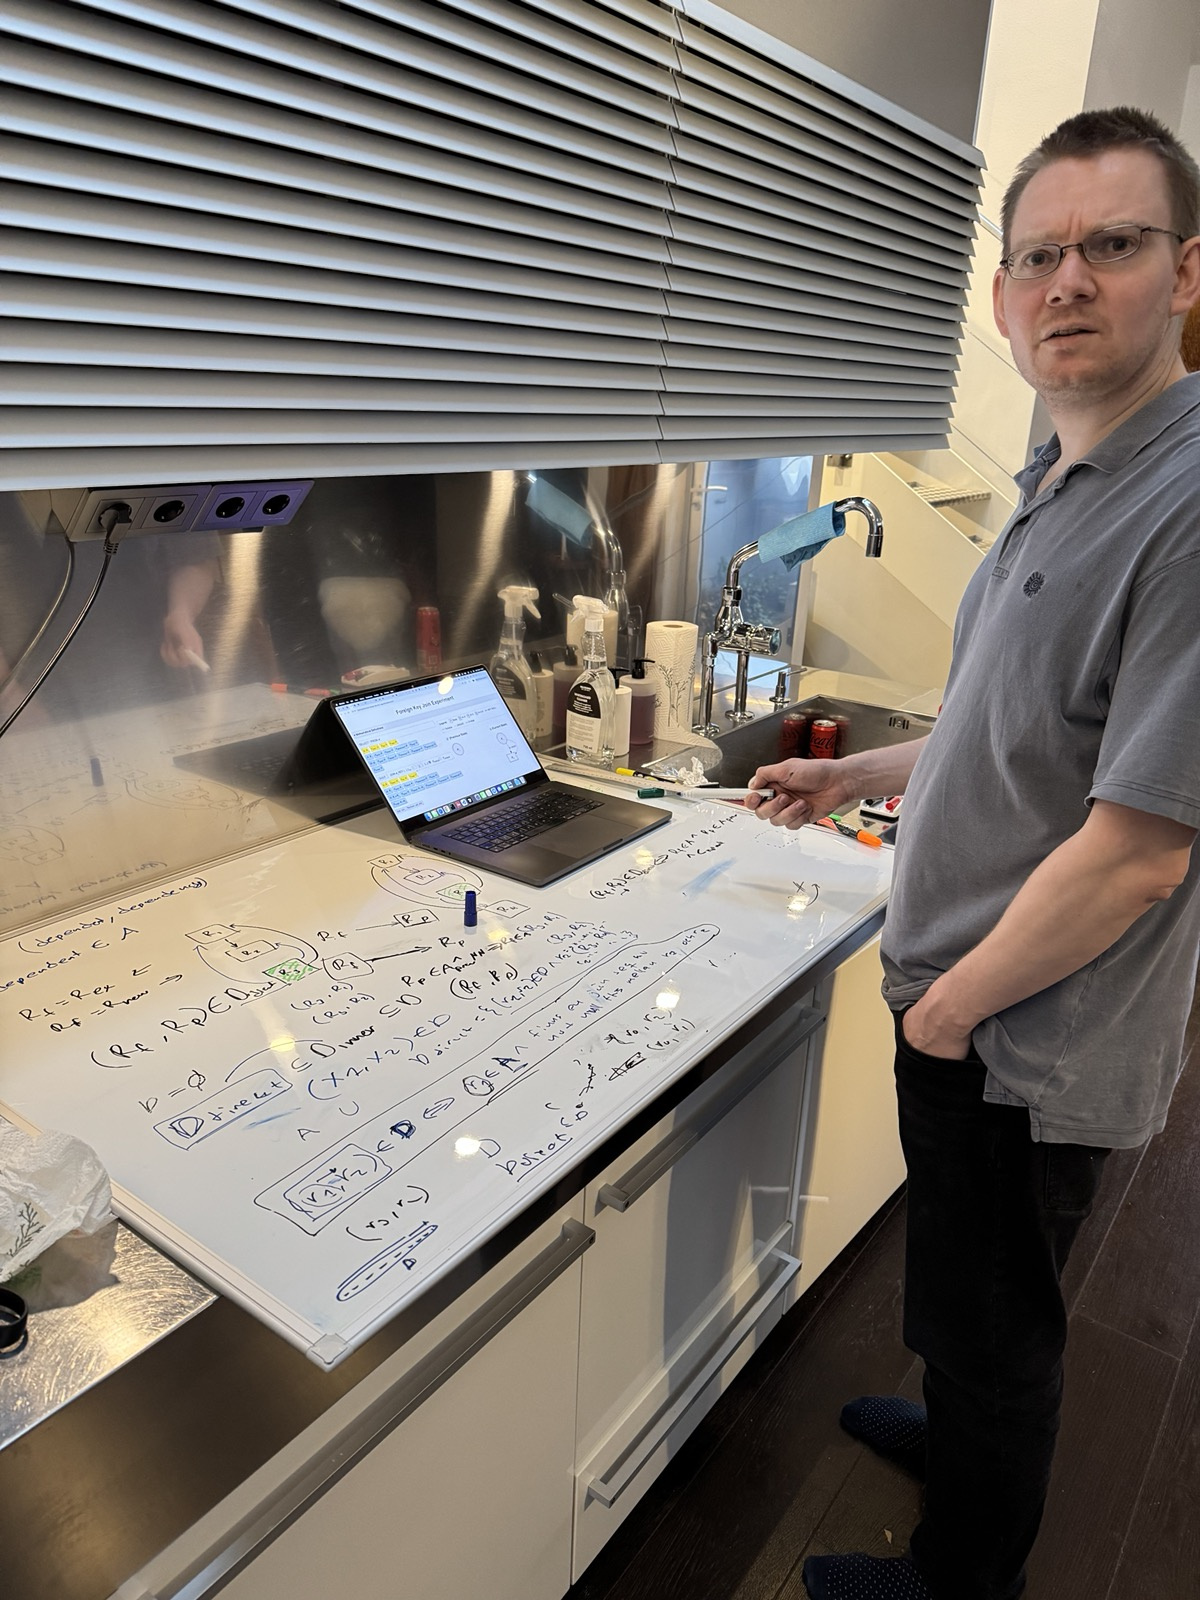
\includegraphics[height=130mm]{assets/key-joins-valencia/derived-tables-workshop.jpg}}
\newcommand{\KeyJoinsPhotoTwo}{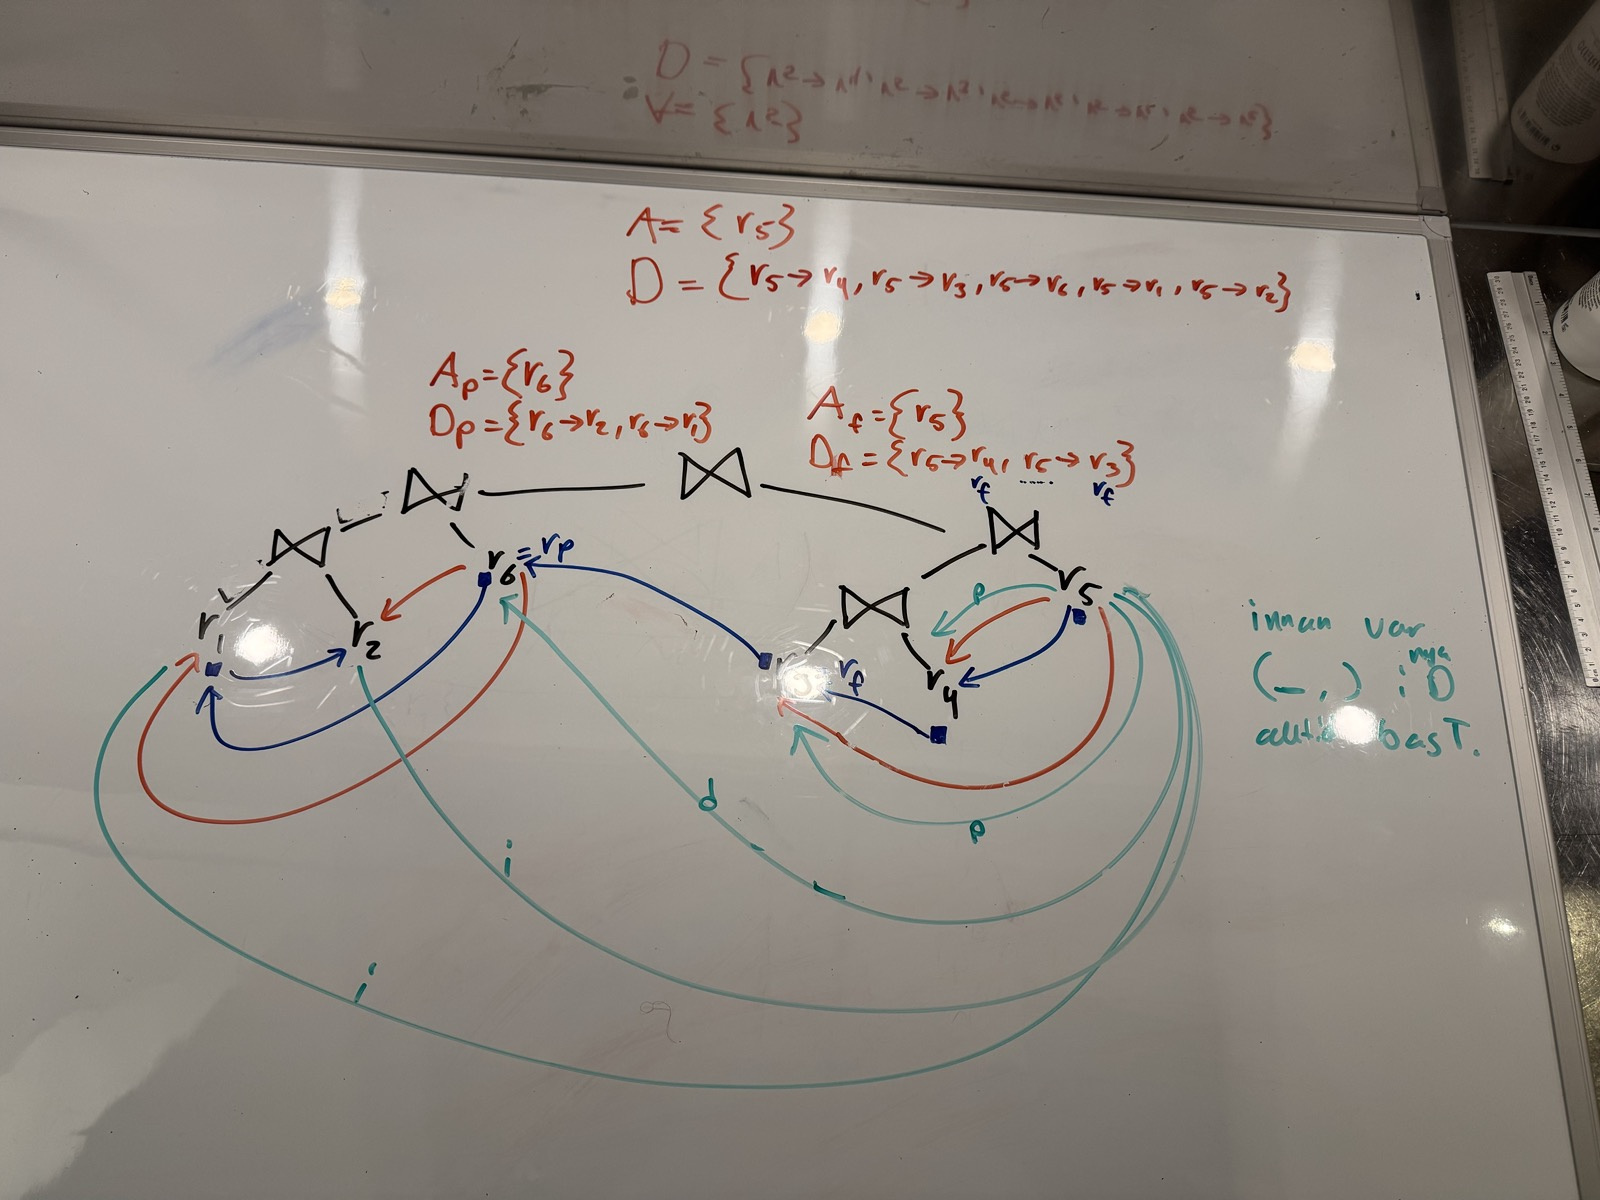
\includegraphics[height=130mm]{assets/key-joins-valencia/derived-tables-whiteboard.jpg}}
% Stockholm group photograph, supplied as IMG_5187.HEIC.
% Full original dimensions and proportions; no crop.
\newcommand{\KeyJoinsStockholmPhoto}{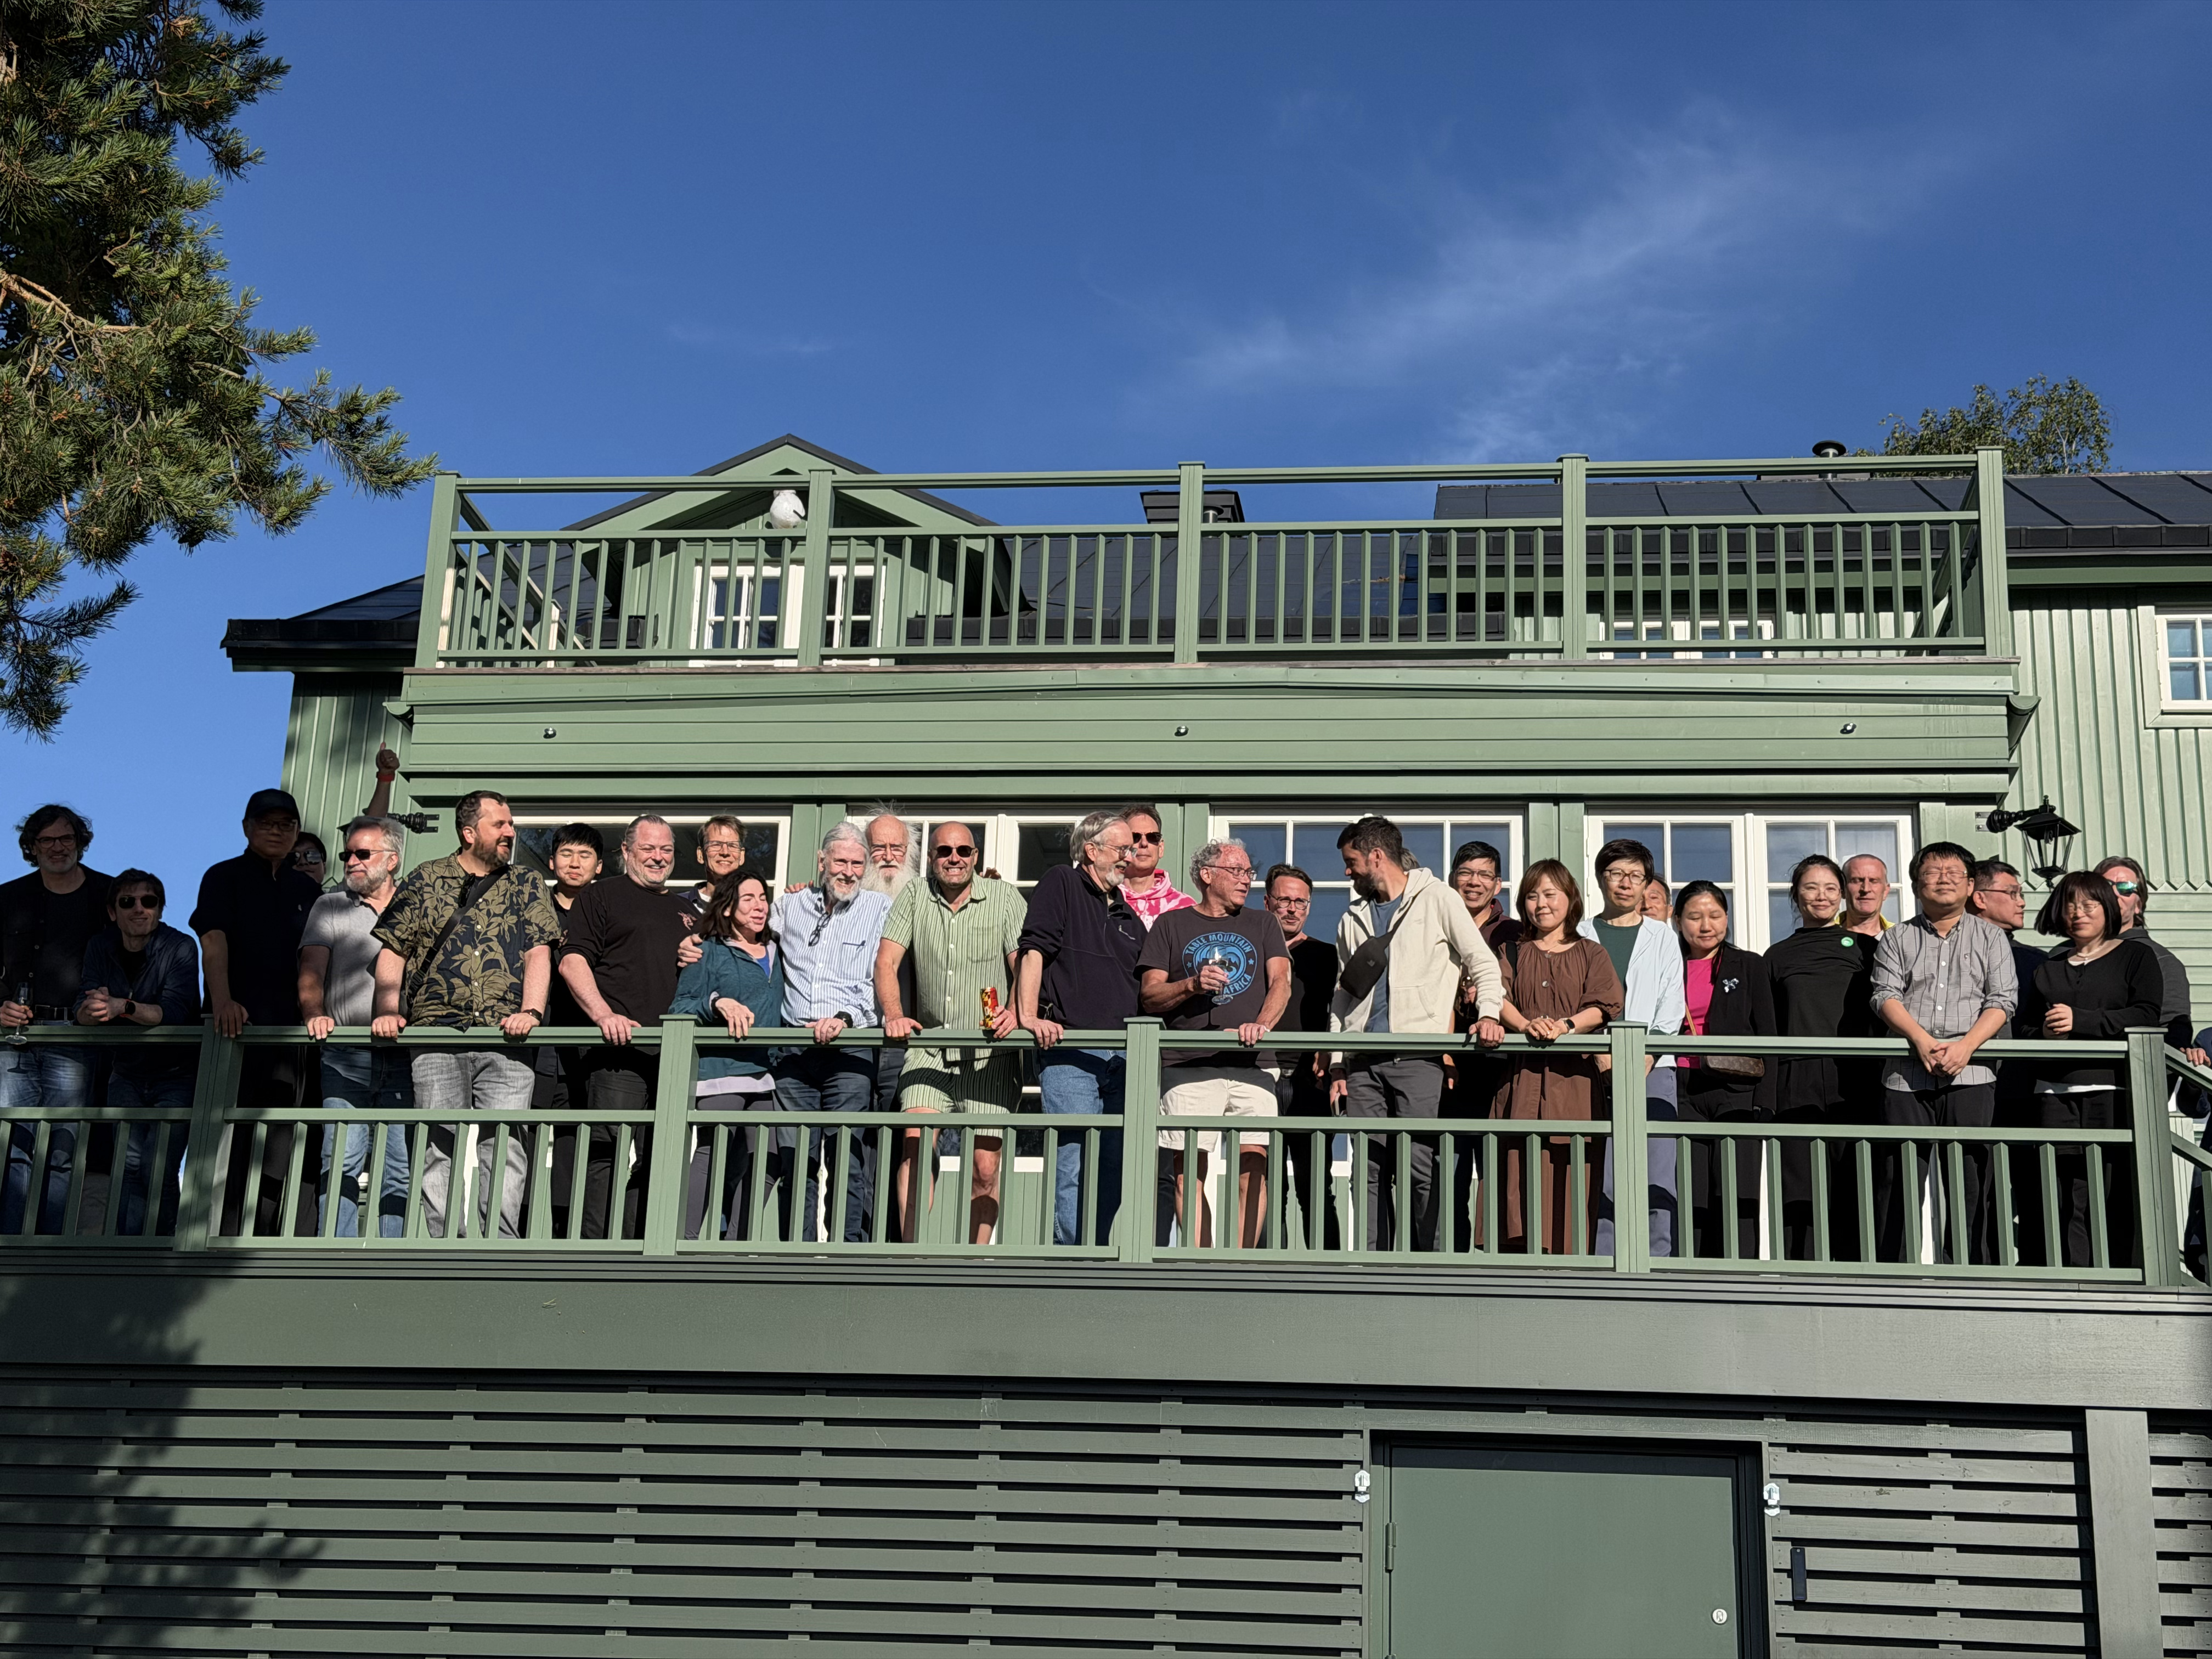
\includegraphics[width=168mm]{assets/key-joins-valencia/stockholm.jpg}}
% Standardese group photograph supplied by the presenter.
% Original JPEG bytes and proportions retained; no crop.
\newcommand{\KeyJoinsStandardesePhoto}{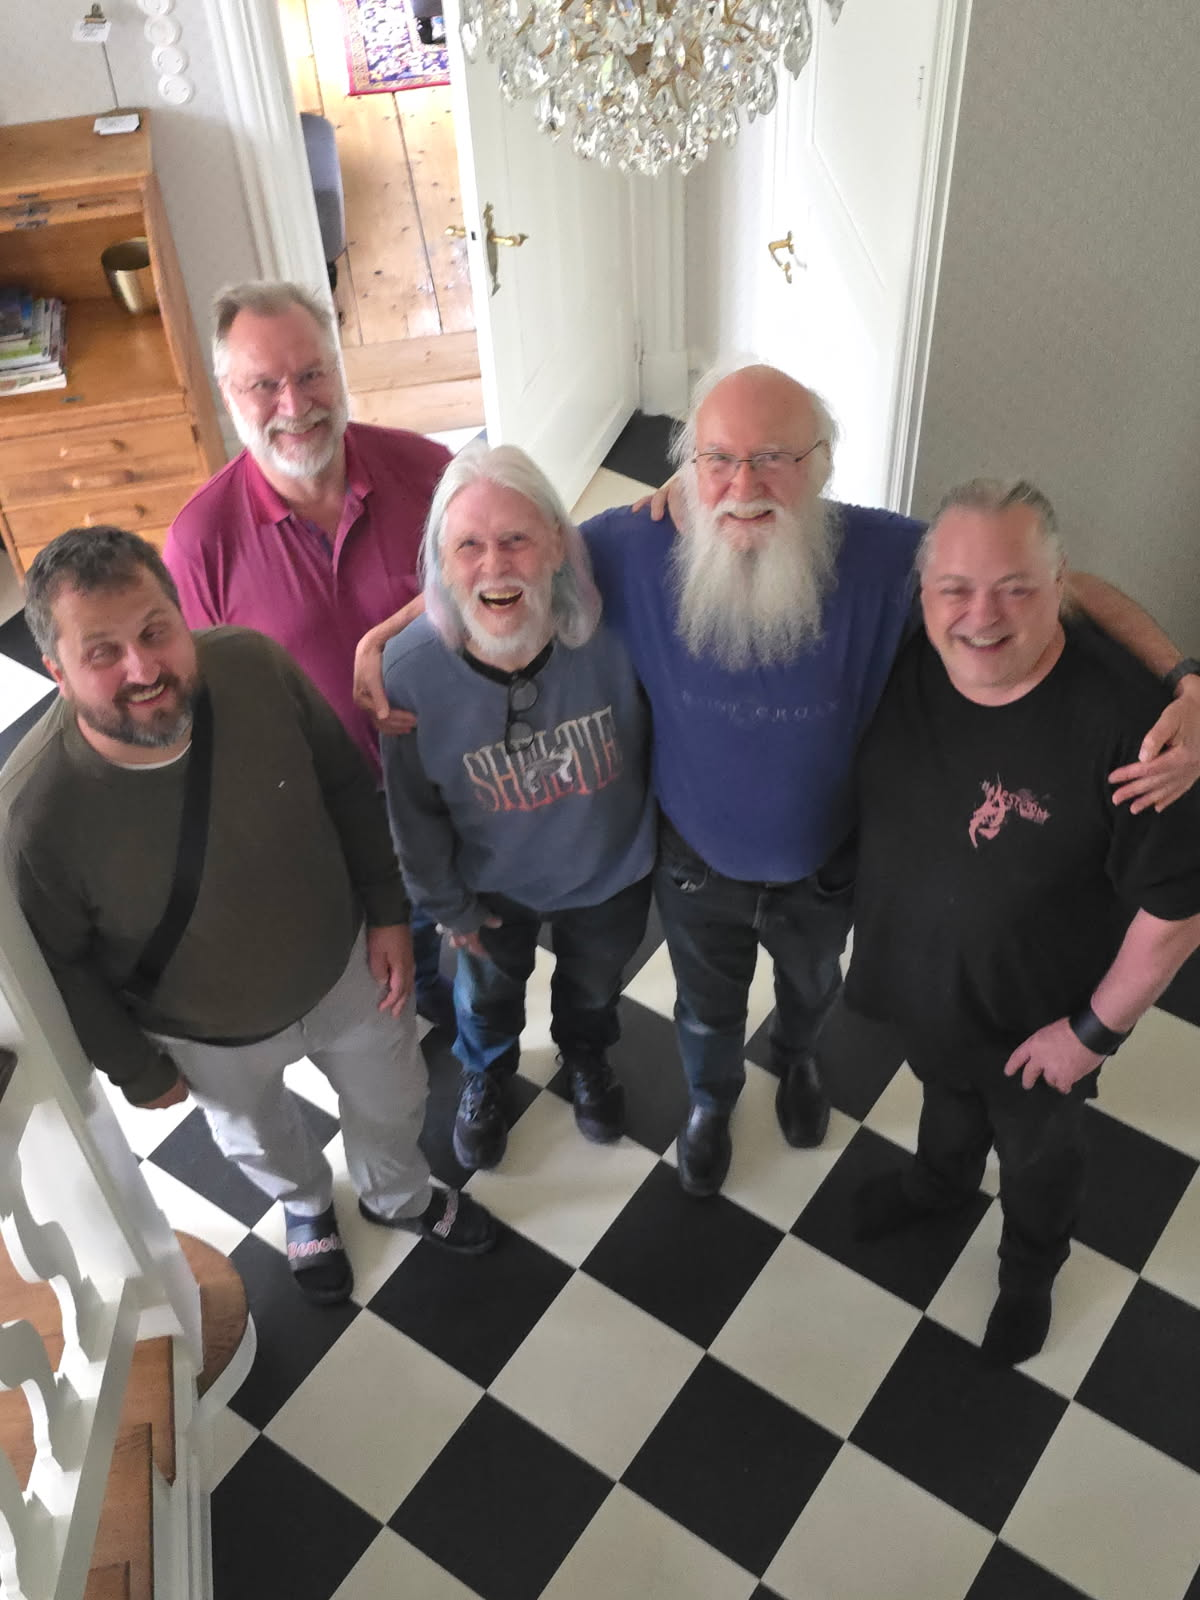
\includegraphics[width=105mm]{assets/key-joins-valencia/standardese-experts.jpg}}
% Photograph supplied for Restarting work with ISO.
% Original dimensions and proportions retained; no crop.
\newcommand{\KeyJoinsISORestartPhoto}{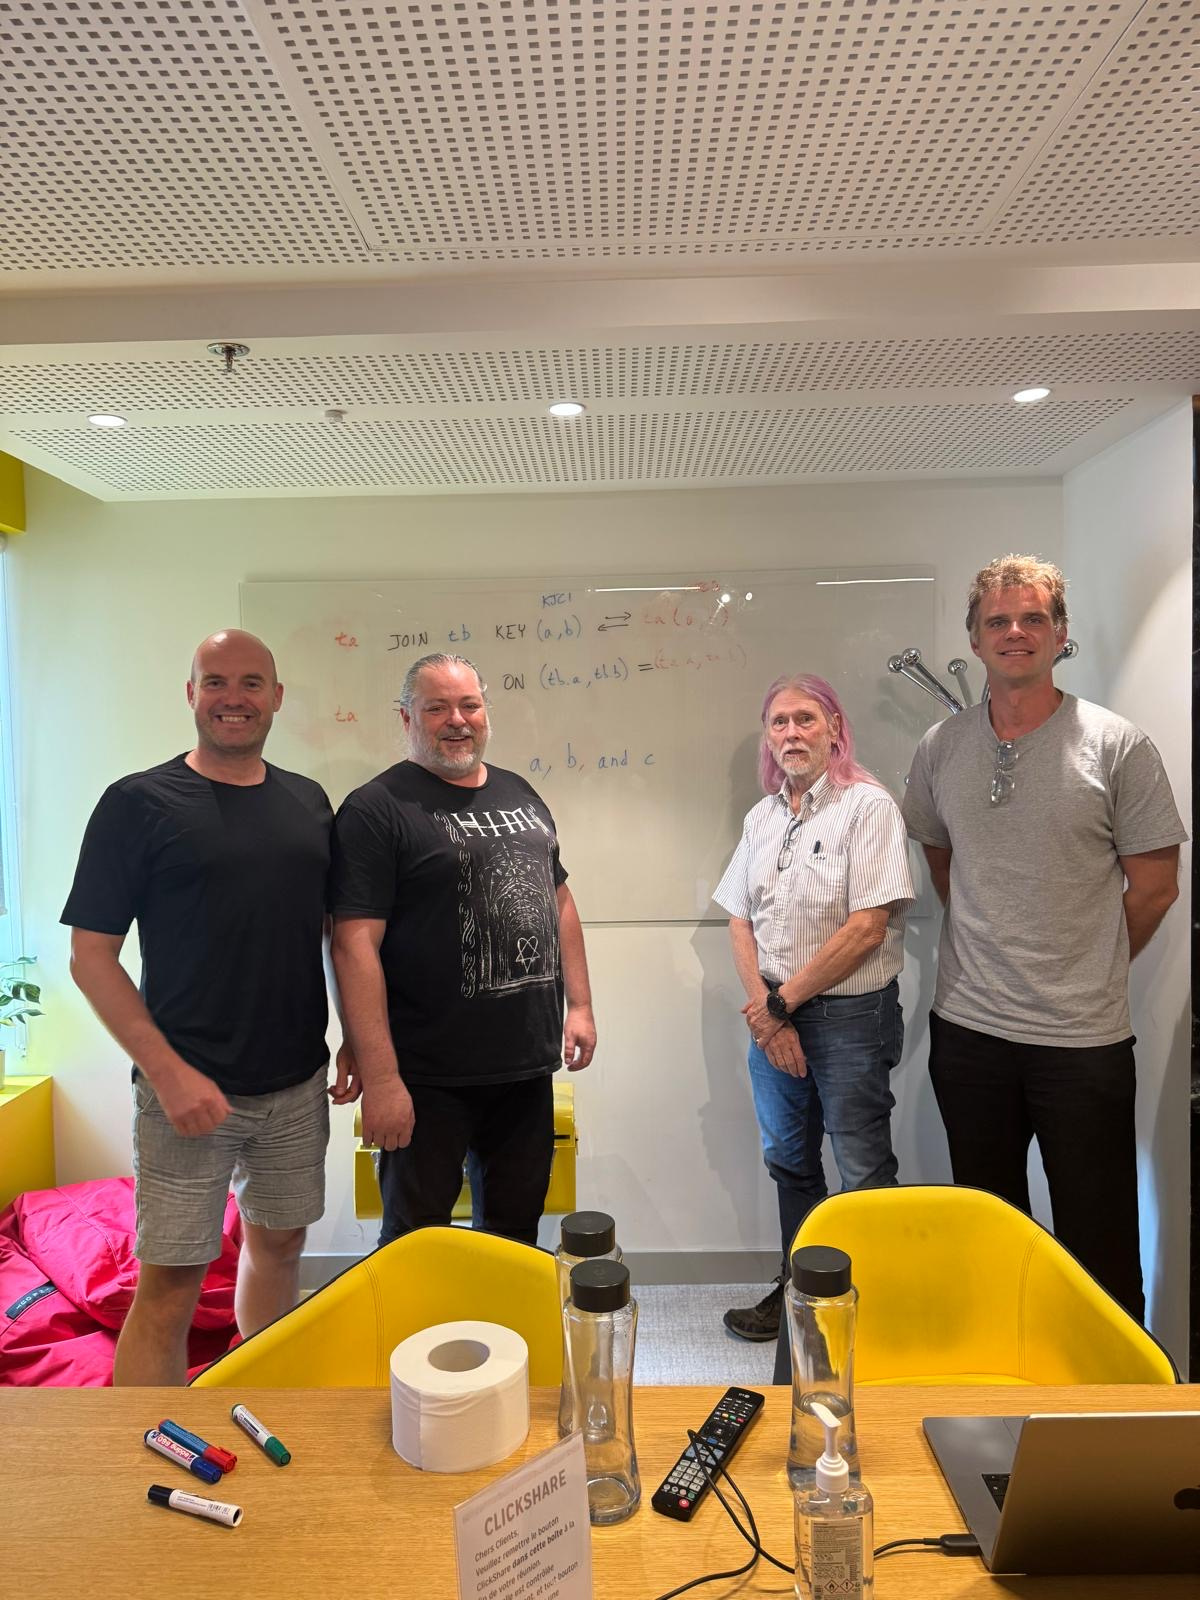
\includegraphics[width=105mm]{assets/key-joins-valencia/restarting-iso.jpg}}
% Acceptance-day photograph: IMG_7395.HEIC, 12 October 2026, confirmed by Joel.
% Full pixel dimensions; camera orientation applied; no crop or resize.
\newcommand{\KeyJoinsAcceptancePhoto}{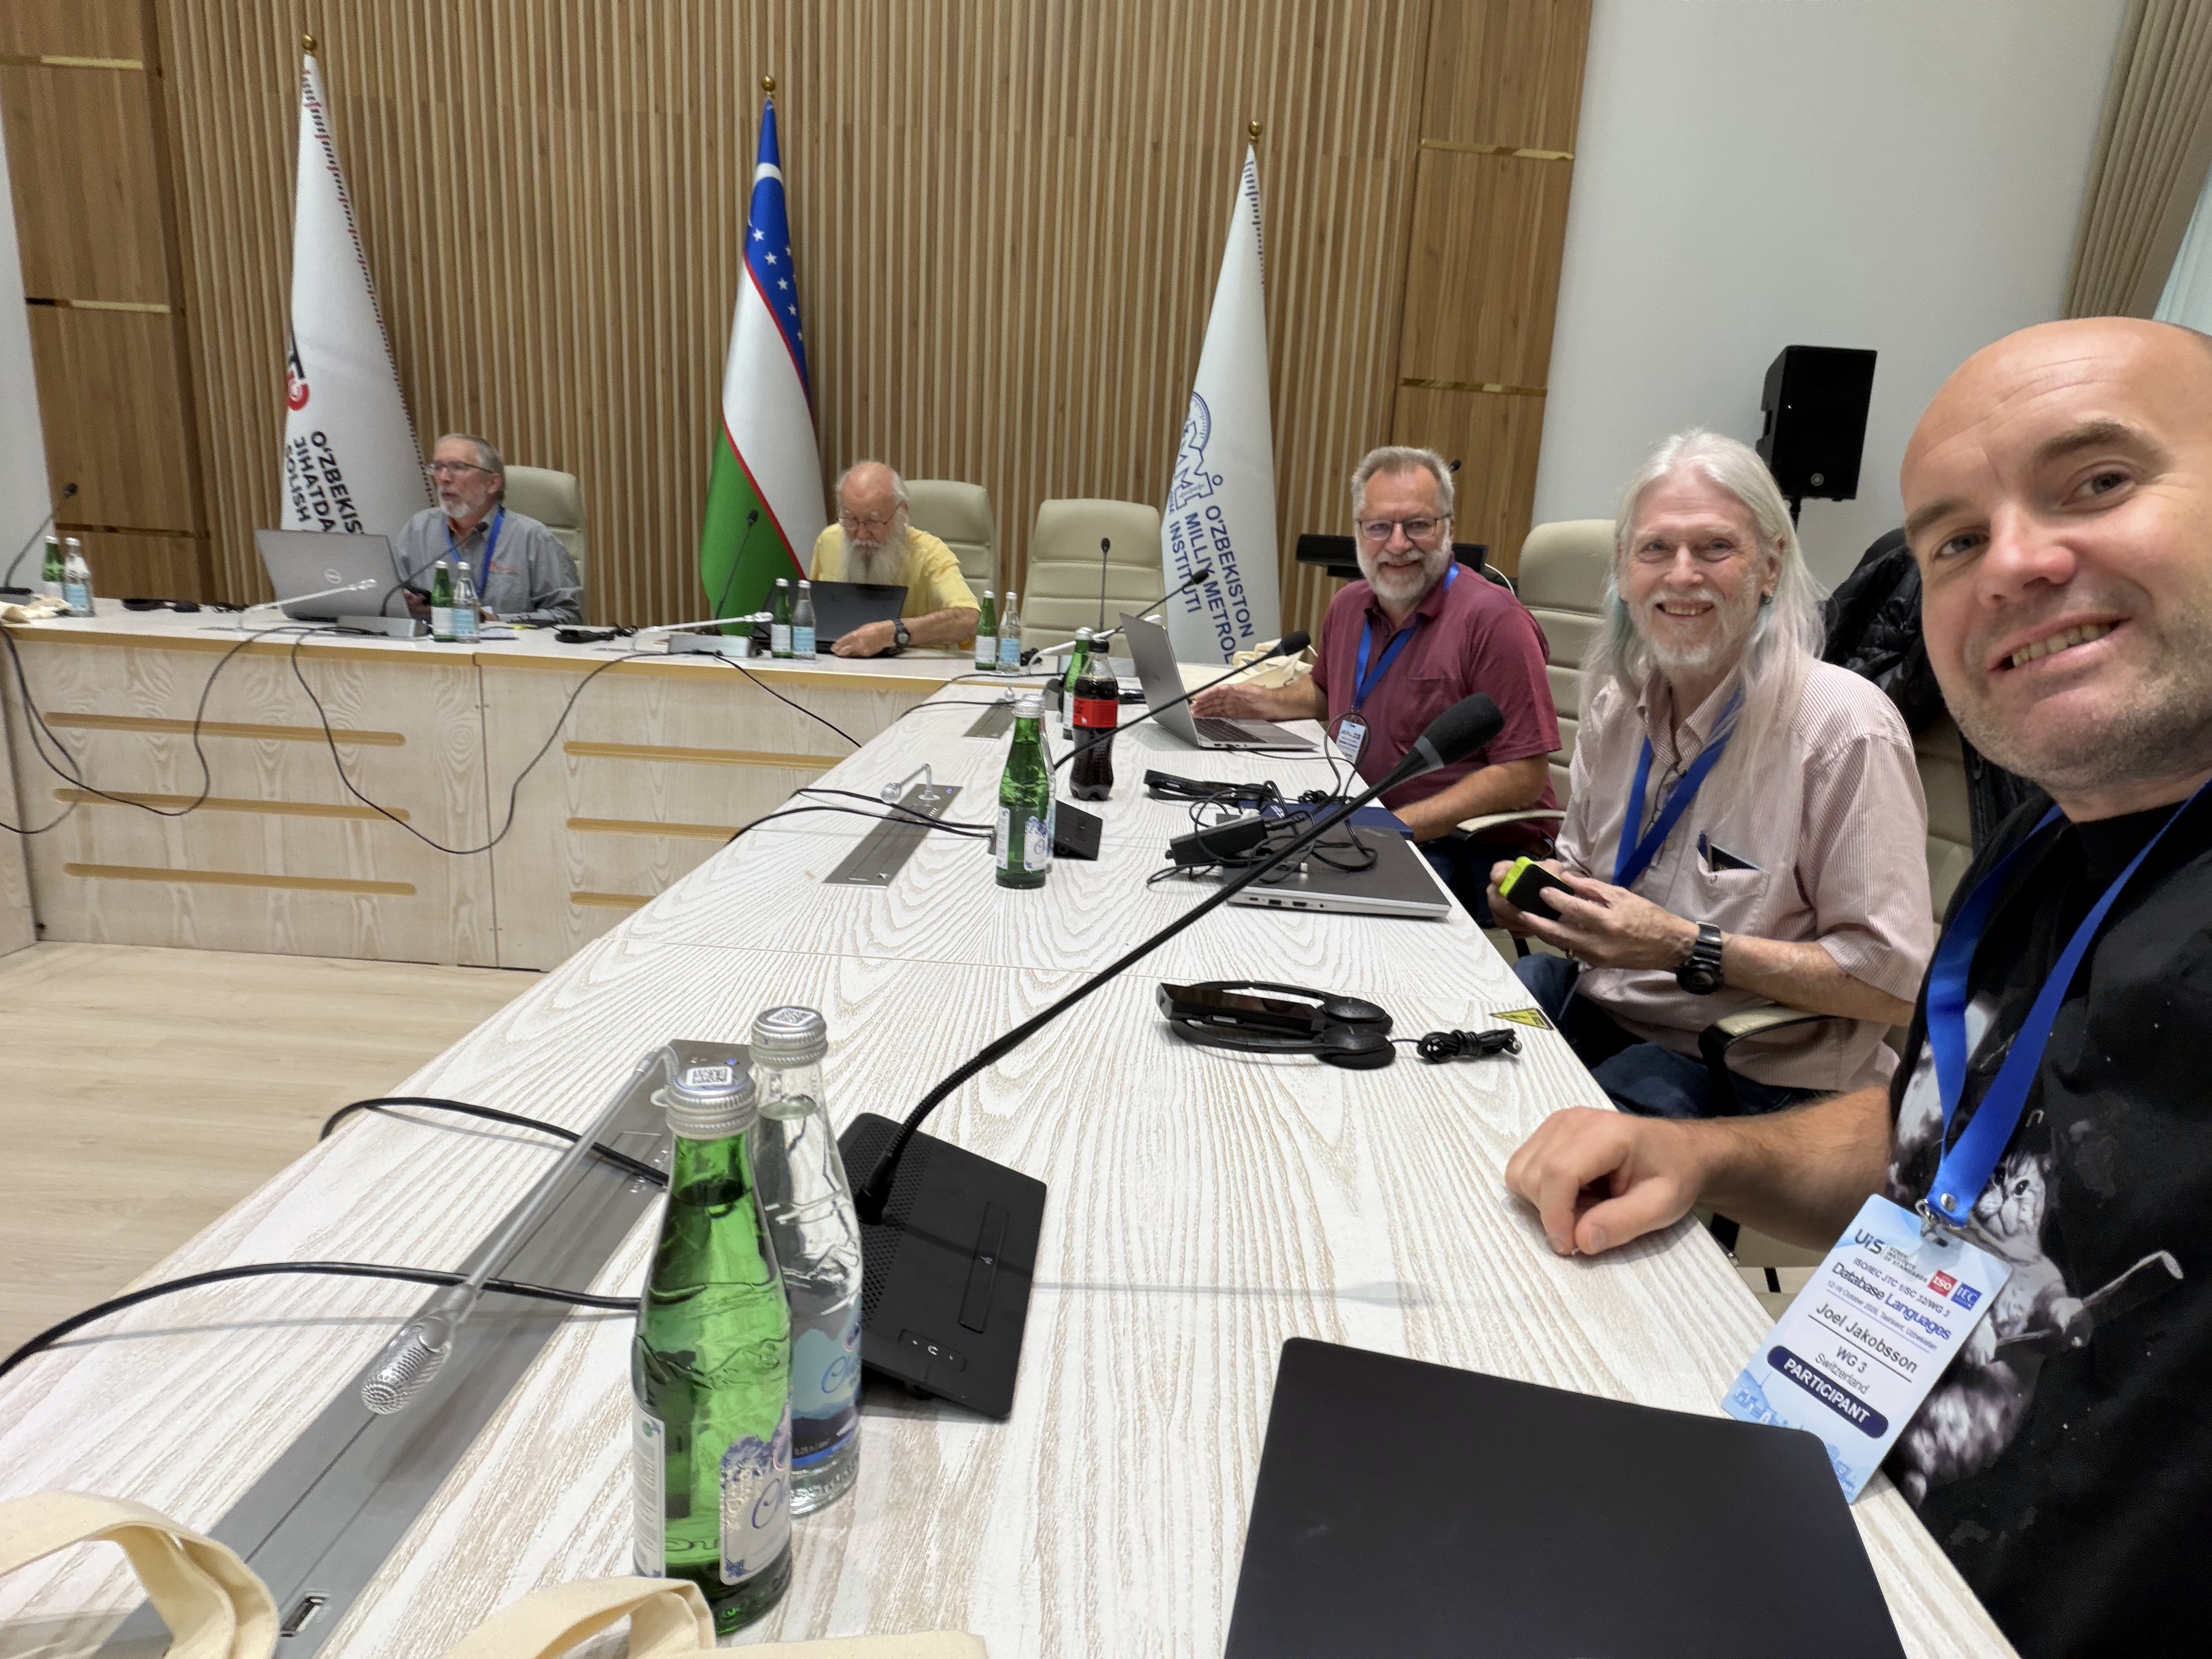
\includegraphics[width=164mm]{assets/key-joins-valencia/tashkent-acceptance.jpg}}

% Mimer logo (vector PDF)
% Official SVG: https://www.mimer.com/wp-content/uploads/logo-mimer-black.svg
% Used with permission, confirmed by Joel. Original vector paths, colors and proportions.
\newcommand{\MimerLogo}{\href{https://www.mimer.com/}{
\includegraphics[width=90mm]{assets/key-joins-valencia/mimer-logo.pdf}}}


% Editable vector reconstruction of the historical composability example.
\definecolor{compoBorder}{HTML}{DDDDDD}
\definecolor{compoCode}{HTML}{F6F8FA}
\definecolor{compoKeyword}{HTML}{0550AE}
\definecolor{compoText}{HTML}{1A1A1A}
\definecolor{compoGood}{HTML}{1A7F37}
\definecolor{compoGoodFill}{HTML}{DAFBE1}
\definecolor{compoBad}{HTML}{CF222E}
\definecolor{compoBadFill}{HTML}{FFEBE9}
\lstdefinestyle{composability-sql}{
  style=fanout-mono,language=SQL,morekeywords={FOR,KEY},
  basicstyle=\ttfamily\fontsize{15.5}{22}\selectfont\color{compoText},
  keywordstyle=\color{compoKeyword}\bfseries
}
\lstdefinestyle{composability-message}{
  style=fanout-mono,
  basicstyle=\ttfamily\fontsize{14.5}{19}\selectfont\color{compoText}
}
\newsavebox{\composabilityView}
\newsavebox{\composabilityInline}
\newsavebox{\composabilityError}
\newsavebox{\composabilityAccepted}

\begin{document}

\begin{lrbox}{\composabilityView}\begin{minipage}{158mm}
\begin{lstlisting}[style=composability-sql]
CREATE VIEW v AS
  SELECT orders.id AS order_id
  FROM order_items
  JOIN orders FOR KEY (id) <- order_items (order_id);

SELECT * FROM v
JOIN payments FOR KEY (order_id) -> v (order_id);
\end{lstlisting}
\end{minipage}\end{lrbox}
\begin{lrbox}{\composabilityInline}\begin{minipage}{158mm}
\begin{lstlisting}[style=composability-sql]
SELECT *
FROM order_items
JOIN orders   FOR KEY (id) <- order_items (order_id)
JOIN payments FOR KEY (order_id) -> orders (id);
\end{lstlisting}
\end{minipage}\end{lrbox}
\begin{lrbox}{\composabilityError}\begin{minipage}{158mm}
\begin{lstlisting}[style=composability-message]
ERROR: foreign key join violation
DETAIL: referenced relation does not preserve
uniqueness of keys
\end{lstlisting}
\end{minipage}\end{lrbox}
\begin{lrbox}{\composabilityAccepted}\begin{minipage}{158mm}
\begin{lstlisting}[style=composability-message]
No error. Query compiles and runs.
\end{lstlisting}
\end{minipage}\end{lrbox}
\FanoutCheckHeight{\composabilityView}{56mm}{Composability view SQL}
\FanoutCheckHeight{\composabilityInline}{33mm}{Composability inline SQL}
\FanoutCheckHeight{\composabilityError}{22mm}{Composability error message}

\begin{lrbox}{\fanoutOrders}\begin{minipage}{7.2cm}
\begin{lstlisting}[style=fanout-sql]
SELECT * FROM orders;
\end{lstlisting}
\begin{lstlisting}[style=fanout-mono]
 id
-----
 100
 101
(2 rows)
\end{lstlisting}
\end{minipage}\end{lrbox}
\begin{lrbox}{\fanoutItems}\begin{minipage}{7.2cm}
\begin{lstlisting}[style=fanout-sql]
SELECT * FROM order_items;
\end{lstlisting}
\begin{lstlisting}[style=fanout-mono]
 id | order_id | amount
----+----------+--------
  1 |      100 |  25.00
  2 |      100 |  75.00
  3 |      101 |  30.00
(3 rows)
\end{lstlisting}
\end{minipage}\end{lrbox}
\begin{lrbox}{\fanoutPayments}\begin{minipage}{7.2cm}
\begin{lstlisting}[style=fanout-sql]
SELECT * FROM payments;
\end{lstlisting}
\begin{lstlisting}[style=fanout-mono]
 id | order_id | amount
----+----------+--------
  1 |      100 |  40.00
  2 |      100 |  60.00
  3 |      101 |  30.00
(3 rows)
\end{lstlisting}
\end{minipage}\end{lrbox}

\begin{lrbox}{\fanoutRawOn}\begin{minipage}{11.9cm}
\begin{lstlisting}[style=fanout-sql]
SELECT o.id,
       SUM(oi.amount) AS item_total,
       SUM(p.amount)  AS payment_total
FROM orders AS o
LEFT JOIN order_items AS oi ON oi.order_id = o.id
LEFT JOIN payments    AS p  ON p.order_id  = o.id
GROUP BY o.id;
\end{lstlisting}
\vspace{.25cm}
\begin{lstlisting}[style=fanout-mono]
 id  | item_total | payment_total
-----+------------+---------------
 100 |     200.00 |        200.00
 101 |      30.00 |         30.00
(2 rows)
\end{lstlisting}
\end{minipage}\end{lrbox}

\begin{lrbox}{\fanoutRawKey}\begin{minipage}{13.8cm}
\begin{lstlisting}[style=fanout-sql]
SELECT o.id,
       SUM(oi.amount) AS item_total,
       SUM(p.amount)  AS payment_total
FROM orders AS o
LEFT JOIN order_items AS oi FOR KEY o (id) <- oi (order_id)
LEFT JOIN payments    AS p  FOR KEY o (id) <- p (order_id)
GROUP BY o.id;
\end{lstlisting}
\vspace{.25cm}
\begin{lstlisting}[style=fanout-diagnostic]
ERROR:  key join from referencing relation p to
        referenced relation o cannot be proven
LINE 6: LEFT JOIN payments    AS p  FOR KEY o (id) <- p (order_id)
                                    ^
DETAIL:  Referenced columns o (id) are not proven unique.
         A preceding join may duplicate rows from
         referenced relation o.
\end{lstlisting}
\end{minipage}\end{lrbox}

\begin{lrbox}{\fanoutGroupedOn}\begin{minipage}{11.9cm}
\begin{lstlisting}[style=fanout-sql]
SELECT o.id,
       oi.item_total,
       p.payment_total
FROM orders AS o
LEFT JOIN (
    SELECT order_id, SUM(amount) AS item_total
    FROM order_items
    GROUP BY order_id
) AS oi ON o.id = oi.order_id
LEFT JOIN (
    SELECT order_id, SUM(amount) AS payment_total
    FROM payments
    GROUP BY order_id
) AS p ON o.id = p.order_id;
\end{lstlisting}
\vspace{.25cm}
\begin{lstlisting}[style=fanout-mono]
 id  | item_total | payment_total
-----+------------+---------------
 100 |     100.00 |        100.00
 101 |      30.00 |         30.00
(2 rows)
\end{lstlisting}
\end{minipage}\end{lrbox}

\begin{lrbox}{\fanoutGroupedKey}\begin{minipage}{13.8cm}
\begin{lstlisting}[style=fanout-sql]
SELECT o.id,
       oi.item_total,
       p.payment_total
FROM orders AS o
LEFT JOIN (
    SELECT order_id, SUM(amount) AS item_total
    FROM order_items
    GROUP BY order_id
) AS oi FOR KEY o (id) <- oi (order_id)
LEFT JOIN (
    SELECT order_id, SUM(amount) AS payment_total
    FROM payments
    GROUP BY order_id
) AS p FOR KEY o (id) <- p (order_id);
\end{lstlisting}
\vspace{.25cm}
\begin{lstlisting}[style=fanout-mono]
 id  | item_total | payment_total
-----+------------+---------------
 100 |     100.00 |        100.00
 101 |      30.00 |         30.00
(2 rows)
\end{lstlisting}
\end{minipage}\end{lrbox}
\FanoutCheckHeight{\fanoutOrders}{35mm}{Orders data}
\FanoutCheckHeight{\fanoutItems}{40mm}{Order items data}
\FanoutCheckHeight{\fanoutPayments}{40mm}{Payments data}
\FanoutCheckHeight{\fanoutRawOn}{124mm}{Original ON query}
\FanoutCheckHeight{\fanoutRawKey}{124mm}{Original FOR KEY query}
\FanoutCheckHeight{\fanoutGroupedOn}{124mm}{Corrected ON query}
\FanoutCheckHeight{\fanoutGroupedKey}{124mm}{Corrected FOR KEY query}



% 1. Designing a new SQL language feature
% Presenter note: Open with the outcome: WG3 agreed to accept the proposal in Tashkent. This talk is the story of how the feature changed, not a tutorial on every rule.
% The recording identifies Joel and Andreas as the presenters. Use Joel Jacobson, the international spelling he uses in the PostgreSQL community.
\begin{slide}{1}{PGConf.EU \textperiodcentered{} Valencia \textperiodcentered{} 20 October 2026}{Designing a new SQL language feature}{PGConf.EU 2026 \textperiodcentered{} Designing a new SQL language feature: Key joins}{1 / 34}
\pdfbookmark[0]{Designing a new SQL language feature}{slide-1}
\txt{18}{83}{364}{63}{77.5}{ink}{\textbf{Key joins}}
\txt{20}{125}{350}{27}{33.2}{muted}{Five years from an idea to an SQL feature}
\draw[blue,line width=1.3pt] (20,154) -- (380,154);
\txt{20}{168}{350}{24}{29.5}{ink}{Andreas Karlsson  \textperiodcentered{}  Joel Jacobson}
\end{slide}

% 2. Who are we?
% Presenter note: Recording 00:00–01:25. Both of us have written and reviewed large SQL queries, stored procedures, layered CTEs and views. That is the practical reason we care. Keep personal introductions short; this is not a CV slide.
\begin{slide}{2}{Application queries brought us here}{Who are we?}{Presenters\textquoteright{} account; PGConf.EU session listing}{2 / 34}
\pdfbookmark[0]{Who are we?}{slide-2}
\txt{18}{77}{171}{34}{41}{blue}{\textbf{Andreas Karlsson}}
\txt{211}{77}{171}{34}{41}{blue}{\textbf{Joel Jacobson}}
\txt{18}{98}{171}{21}{26}{muted}{Percona}
\txt{211}{98}{171}{21}{26}{muted}{SQL StdDev AB}
\draw[rulecolor,line width=1pt] (18,126) -- (382,126);
\txt{18}{145}{364}{27}{34}{ink}{Application developers. PostgreSQL contributors.\\[5mm]ISO/IEC JTC 1/SC 32/WG 3 committee members.}
\end{slide}

% 3. What will this talk be about?
% Presenter note: Recording 01:27–06:17. Signal the promised story: proposals that did not work, community feedback, implementation and committee collaboration. Acceptance is the coauthors’ first-hand report of the TAS meeting, not a claim that a new ISO edition has already been published.
% The prepared talk is timed separately in this guide; leave time for questions.
\begin{slide}{3}{One idea, many revisions}{What will this talk be about?}{2021 mailing-list discussion; WG3 papers; presenters\textquoteright{} account of TAS}{3 / 34}
\pdfbookmark[0]{What will this talk be about?}{slide-3}
\txt{18}{80}{100}{37}{45.5}{blue}{2021}
\txt{18}{103}{103}{25}{30.8}{ink}{A shorter way\\to write joins}
\txt{149}{80}{100}{37}{45.5}{blue}{2024\textendash{}2026}
\txt{149}{103}{106}{25}{30.8}{ink}{From shorthand\\to guarantees}
\txt{280}{80}{100}{37}{45.5}{teal}{October 2026}
\txt{280}{103}{105}{25}{30.8}{ink}{Key Joins\\accepted by WG3}
\draw[blue,line width=1.5pt,-{Stealth[length=3mm]}] (120,103) -- (140,103);
\draw[blue,line width=1.5pt,-{Stealth[length=3mm]}] (255,103) -- (272,103);
\end{slide}

% 4. What are key joins?
% Presenter note: Replaces the introductory employees/departments example (recording 03:11–06:17) with the fanout example. Assume orders.id is a primary key and both order_id columns are NOT NULL foreign keys to it, with enforced, non-deferrable constraints. The ON query repeats each item for each payment, and each payment for each item: order 100 has four intermediate rows, so both sums are 200 instead of 100. The first FOR KEY join is valid: every referencing item has one matching order. The second is rejected because o.id is no longer unique in the complete left operand. FOR KEY does not repair the query or prove the whole query correct.
% Omit the tentative BEAVER percentages from the recording: they were explicitly awaiting verification.
% ERROR and DETAIL are wrapped without changing their wording. LINE 6 matches the displayed query; its diagnostic caret has 36 leading spaces. Displayed row order is illustrative, since the queries have no ORDER BY.
\begin{slide}{4}{Double-counting from join fanout}{What are key joins?}{Example inspired by Paul Jungwirth: \href{https://www.postgresql.org/message-id/flat/86b9ec78-925c-1935-bc9d-6bad4ceb1f40@illuminatedcomputing.com}{\textcolor{blue}{Avoiding double-counting in aggregates with more than one join?}} \textperiodcentered{} pgsql-general, 2016}{4 / 34}
\pdfbookmark[0]{What are key joins? -- Double-counting from join fanout}{slide-4}
\FanoutBody{\fanoutRawOn}{\fanoutRawKey}
\end{slide}

% 5. What are key joins?
% Presenter note: Aggregate each many side by order_id before joining it to orders. Each grouped result has at most one row per order, so the first join leaves o.id unique for the second join. The same NOT NULL foreign keys supply the relationship and coverage facts through the grouping. Both ON and FOR KEY return 100/100 for order 100 and 30/30 for order 101. FOR KEY makes the DBMS check each join; the query author still chooses where to aggregate. The table contents stay in exactly the same positions as on the preceding page.
\begin{slide}{5}{Aggregating before joining}{What are key joins?}{Example inspired by Paul Jungwirth: \href{https://www.postgresql.org/message-id/flat/86b9ec78-925c-1935-bc9d-6bad4ceb1f40@illuminatedcomputing.com}{\textcolor{blue}{Avoiding double-counting in aggregates with more than one join?}} \textperiodcentered{} pgsql-general, 2016}{5 / 34}
\pdfbookmark[0]{What are key joins? -- Aggregating before joining}{slide-4-corrected}
\FanoutBody{\fanoutGroupedOn}{\fanoutGroupedKey}
\end{slide}

% 6. Joel’s first idea
% Presenter note: Recording 06:17–08:57. Joel saw Neo4j’s SQL/Cypher comparison and mistakenly assumed its arrows meant foreign-key references. That misunderstanding inspired the idea. This exact path-expression query is reproduced in the written background and 2021 thread. It was a convenience idea, with the presence of a foreign key as a check; it did not yet have today’s preservation contract.
% Source: https://www.postgresql.org/message-id/flat/CAMsGm5eeDXFX7oA9H6hF0E%2BaZZP4D8nbChtt_3BSotGPLXshNQ%40mail.gmail.com
\begin{slide}{6}{27 March 2021 \textperiodcentered{} Inspired by Cypher}{Joel\textquoteright{}s first idea}{pgsql-hackers, March 2021 \textperiodcentered{} \textquotedblleft{}Avoid JOINs by using path expressions to follow FKs\textquotedblright{}}{6 / 34}
\pdfbookmark[0]{Joel\textquoteright{}s first idea}{slide-5}
\txt{18}{76}{350}{14.5}{17.8}{blue}{\textbf{COULD SQL FOLLOW FOREIGN KEYS WITH PATH EXPRESSIONS?}}
\codeat{18}{95}{22}{28.6}{\textcolor{blue}{\textbf{SELECT}} \textcolor{blue}{\textbf{DISTINCT}} od.order\_id.customer\_id.company\_name\strut \\
\textcolor{blue}{\textbf{FROM}} order\_details \textcolor{blue}{\textbf{AS}} od\strut \\
\textcolor{blue}{\textbf{WHERE}} od.product\_id.product\_name = \textcolor{teal}{'Chocolade'};\strut}
\txt{18}{145}{350}{29}{35.7}{ink}{Fewer comparisons to type.\\Fewer opportunities for a typo.}
\txt{18}{187}{350}{18}{22.1}{orange}{Historical proposal \textemdash{} not PostgreSQL syntax.}
\end{slide}

% 7. Feedback from mailinglist
% Presenter note: Recording 08:57–10:42. Credit the actual argument correctly: Álvaro Herrera raised ambiguity after adding a foreign key; Tom Lane explained the dependency problem and the composite-key issue. Andrew Dunstan and Pavel Stehule objected to hiding joins. Pantelis Theodosiou discussed intermediate results and repeated paths.
% Joel initially defended the idea by comparing it to USING/NATURAL. In retrospect, an existing awkward feature is not a good reason to add another. Keep this self-critical rather than dismissing the feedback.
\begin{slide}{7}{Late March 2021 \textperiodcentered{} The problems with implicit joins}{Feedback from mailinglist}{pgsql-hackers, March 2021 \textperiodcentered{} Herrera, Lane, Dunstan, Stehule, Theodosiou}{7 / 34}
\pdfbookmark[0]{Feedback from mailinglist}{slide-6}
\txt{18}{78}{170}{27}{33.2}{ink}{What about composite keys?\\[4mm]Which foreign key?}
\txt{211}{78}{171}{27}{33.2}{ink}{What about outer joins?\\[4mm]How many joins did we just write?}
\draw[rulecolor,line width=1pt] (18,142) -- (382,142);
\txt{18}{157}{350}{29}{35.7}{orange}{Adding a foreign key must not make\\an existing query ambiguous.}
\end{slide}

% 8. Proposal from Vik
% Presenter note: Recording 10:42–13:02. Vik’s concrete alternative mattered more than his “terrible idea” opening. The WITH example is the historical suggestion, not final syntax. It also handles multi-column foreign keys. Andreas recalls this as the point where he became interested. Vik’s insistence on working with the SQL standard shaped the next step.
% Quotes verified against Vik's public messages of 28 March (two different replies) and 31 March 2021. The first concerns the implicit-path idea; the last agrees with Pavel about avoiding proprietary syntax. Preserve the original capitalized Standard. The dates in the footer link to the three original messages.
\begin{slide}{8}{28\textendash{}31 March 2021 \textperiodcentered{} Keep the join explicit}{Proposal from Vik}{Vik Fearing, pgsql-hackers: \href{https://www.postgresql.org/message-id/f2eff805-69ec-4968-788c-053abd32b168@postgresfriends.org}{28 March (first reply)}; \href{https://www.postgresql.org/message-id/f5770a13-61a6-603e-6a66-14c65eea9998@postgresfriends.org}{28 March (follow-up)}; \href{https://www.postgresql.org/message-id/e1e3b3d1-d337-db15-71c9-d1e4da6f5e9c@postgresfriends.org}{31 March 2021}}{8 / 34}
\pdfbookmark[0]{Proposal from Vik}{slide-7}
\txt{18}{77}{364}{27}{34}{ink}{\textquotedblleft{}This is a terrible idea, but let me explain why.\textquotedblright{}}
\txt{18}{111}{364}{27}{34}{ink}{\textquotedblleft{}SQL is not an implicit language, though.\textquotedblright{}}
\codeat{18}{135}{25}{32.5}{\textcolor{blue}{\textbf{FROM}} a \textcolor{blue}{\textbf{JOIN}} b \textcolor{blue}{\textbf{WITH}} a\_b\_fk\strut}
\txt{18}{166}{364}{27}{34}{ink}{\textquotedblleft{}I'm with you on this: let's do it the Standard way,\\or not do it at all.\textquotedblright{}}
\end{slide}

% 9. Syntax bikeshedding
% Presenter note: Recording 13:02–14:36. Introduce Anders Granlund as an early coauthor. The keywords on screen are successive ideas, not an exhaustive chronological list and not all from a single paper. The first WITH is Vik's March suggestion; JOIN WITH is Joel's fully spelled-out December 28 proposal; FOREIGN KEY is the January 2022 draft with one referencing-column list; KEY FROM is the later two-list form. Table and constraint names are adapted consistently. Avoid spending the talk arguing which keyword is prettiest.
\begin{slide}{9}{March 2021\textendash{}May 2022 \textperiodcentered{} With Anders Granlund, the mailing list and Hacker News}{Syntax bikeshedding}{Historical forms, with names adapted \textperiodcentered{} March and December 2021 correspondence; January and May 2022 drafts}{9 / 34}
\pdfbookmark[0]{Syntax bikeshedding}{slide-8}
\txt{18}{74}{364}{13}{16}{muted}{MARCH 2021}
\codeat{18}{85}{23}{29.9}{\textcolor{blue}{\textbf{JOIN}} departments \textcolor{blue}{\textbf{AS}} d \textcolor{blue}{\textbf{WITH}} employees\_dept\_id\_fkey\strut}
\txt{18}{106}{364}{13}{16}{muted}{DECEMBER 2021}
\codeat{18}{117}{23}{29.9}{\textcolor{blue}{\textbf{JOIN}} \textcolor{blue}{\textbf{WITH}} e.employees\_dept\_id\_fkey d\strut}
\txt{18}{138}{364}{13}{16}{muted}{JANUARY 2022}
\codeat{18}{149}{23}{29.9}{\textcolor{blue}{\textbf{JOIN}} departments \textcolor{blue}{\textbf{AS}} d \textcolor{blue}{\textbf{FOREIGN}} \textcolor{blue}{\textbf{KEY}} (dept\_id) \textcolor{blue}{\textbf{FROM}} e\strut}
\txt{18}{170}{364}{13}{16}{muted}{TWO COLUMN LISTS}
\codeat{18}{181}{23}{29.9}{\textcolor{blue}{\textbf{JOIN}} departments \textcolor{blue}{\textbf{AS}} d \textcolor{blue}{\textbf{KEY}} (id) \textcolor{blue}{\textbf{FROM}} e (dept\_id)\strut}
\end{slide}

% 10. Why does constraint names not work?
% Presenter note: Recording 14:36–15:55. Keep the user’s exact title. This teaching example uses two instances of employees, each carrying the same declared dept_id foreign key. A derived table is a query result, such as a view or subquery. The base constraint name alone cannot choose between employee_dept_id and manager_dept_id at this surface. One could design more syntax to resolve this, but a bare name is not enough. This is the specific repeated-base-table issue documented in POS-009 p.3.
% The JOIN WITH form adapts Joel's December 28, 2021 example, the latest fully spelled-out constraint-name proposal found before the January draft. Later replies also floated incomplete USING KEY/FOREIGN KEY forms. The orange name is known but does not select employee_dept_id versus manager_dept_id. Do not claim all conceivable constraint-name designs are impossible, or that constraint names must be globally unique.
\begin{slide}{10}{Late 2021\textendash{}early 2022 (approx.) \textperiodcentered{} A declaration is not a column occurrence}{Why does constraint names not work?}{\href{https://www.postgresql.org/message-id/a9a9c45b-7c90-45dc-bdcf-7b3b32a97d41@www.fastmail.com}{JOIN WITH proposal, 28 December 2021}; POS-009, p. 3 \textperiodcentered{} adapted example}{10 / 34}
\pdfbookmark[0]{Why does constraint names not work?}{slide-9}
\codeat{18}{74}{21}{27.3}{\textcolor{blue}{\textbf{CREATE}} \textcolor{blue}{\textbf{VIEW}} staff \textcolor{blue}{\textbf{AS}}\strut \\
\textcolor{blue}{\textbf{SELECT}} e.dept\_id \textcolor{blue}{\textbf{AS}} employee\_dept\_id,\strut \\
\hspace*{3.675em}m.dept\_id \textcolor{blue}{\textbf{AS}} manager\_dept\_id\strut \\
\textcolor{blue}{\textbf{FROM}} employees \textcolor{blue}{\textbf{AS}} e\strut \\
\textcolor{blue}{\textbf{LEFT}} \textcolor{blue}{\textbf{JOIN}} employees \textcolor{blue}{\textbf{AS}} m \textcolor{blue}{\textbf{ON}} e.manager\_id = m.emp\_id;\strut}
\txt{18}{126}{364}{18}{22}{muted}{Both columns originate from the same foreign key declaration.}
\codeat{18}{145}{22}{28.6}{\textcolor{blue}{\textbf{FROM}} staff \textcolor{blue}{\textbf{AS}} s\strut \\
\textcolor{blue}{\textbf{LEFT}} \textcolor{blue}{\textbf{JOIN}} \textcolor{blue}{\textbf{WITH}} s.\textcolor{orange}{\underline{employees\_dept\_id\_fkey}} d\strut}
\txt{18}{181}{364}{23}{29}{orange}{Which occurrence: \texttt{employee\_dept\_id} or \texttt{manager\_dept\_id}?}
\end{slide}

% 11. Alternative: column lists
% Presenter note: Recording 15:55–16:28. Andreas recalls inspiration from PostgreSQL ON CONFLICT’s ability to identify a unique constraint by columns instead of name. This is an analogy about identifying a relationship; the key-join proof is more involved. The displayed historical syntax follows UTC-107 / CMN-023: the newly joined right table’s list comes first. Later slides will change this.
% Constraint-name syntax was considered, not proved impossible in all conceivable designs.
\begin{slide}{11}{January\textendash{}May 2022 \textperiodcentered{} Identify the columns exposed by the query}{Alternative: column lists}{May 2022 SIS draft, p. 2; UTC-107 and CMN-023 \textperiodcentered{} two explicit column lists}{11 / 34}
\pdfbookmark[0]{Alternative: column lists}{slide-10}
\codeat{18}{80}{25}{32.5}{\textcolor{blue}{\textbf{SELECT}} o.id, c.name\strut \\
\textcolor{blue}{\textbf{FROM}} orders \textcolor{blue}{\textbf{AS}} o\strut \\
\textcolor{blue}{\textbf{JOIN}} customers \textcolor{blue}{\textbf{AS}} c \textcolor{blue}{\textbf{KEY}} (id) \textcolor{blue}{\textbf{FROM}} o (customer\_id);\strut}
\txt{18}{146}{350}{27}{33.2}{ink}{Two lists identify the relationship.\\The DBMS finds the supporting constraint.}
\txt{18}{190}{350}{18}{22.1}{orange}{Historical KEY FROM syntax, with names adapted for this example.}
\end{slide}

% 12. Learning the standards process
% Presenter note: Recording 16:28–19:15. Explain WG3 once: the working group responsible for SQL and related database languages. SIS is the Swedish national standards body. Keith Hare presented UTC-107 at Zeist; the next minutes say it was discussed. Joel and Anders then presented CMN-023 in Casablanca. Jörn and Karl saw practical value; Vik volunteered to help.
% Do not state that nobody responded at UTC as an objective minutes finding. The coauthors’ experience was that the first presentation did not give them a clear next step. Source: W25-001 item 9.2.9; W26-001r1 item 9.2.3.
\begin{slide}{12}{May 2022\textendash{}September 2023 \textperiodcentered{} From Sweden to WG3}{Learning the standards process}{UTC-107 \ensuremath{\rightarrow} W25-001; CMN-023R3 \ensuremath{\rightarrow} W26-001R1}{12 / 34}
\pdfbookmark[0]{Learning the standards process}{slide-11}
\txt{18}{80}{350}{14.5}{17.8}{blue}{\textbf{2022 \textperiodcentered{} SWEDEN}}
\txt{18}{97}{108}{26}{32.0}{ink}{A proposal sent\\to SIS}
\txt{147}{80}{350}{14.5}{17.8}{blue}{\textbf{FEBRUARY 2023 \textperiodcentered{} UTC}}
\txt{147}{97}{109}{26}{32.0}{ink}{Keith presents\\UTC-107}
\txt{277}{80}{350}{14.5}{17.8}{blue}{\textbf{SEPTEMBER 2023 \textperiodcentered{} CMN}}
\txt{277}{97}{108}{26}{32.0}{ink}{Joel and Anders\\present CMN-023}
\draw[blue,line width=1.3pt,-{Stealth[length=3mm]}] (122,116) -- (140,116);
\draw[blue,line width=1.3pt,-{Stealth[length=3mm]}] (252,116) -- (270,116);
\txt{18}{159}{350}{27}{33.2}{ink}{Vik offers to help. Karl and Jörn see the use case.}
\txt{18}{191}{350}{18}{22.1}{muted}{Submitting a paper was only the beginning.}
\end{slide}

% 13. Sidetrack: the MATCH predicate
% Presenter note: Recording 19:15–22:01. The MATCH predicate is distinct from a foreign key’s MATCH type. The idea was to build on it to simplify the change proposal, but it did not settle the intended null behavior. This was an internal exploration, not a released implementation. Ordinary equality does not match a null component. We return to the nullability breakthrough later. No need to teach MATCH PARTIAL here or claim no DBMS has ever implemented the predicate.
\begin{slide}{13}{Late 2023\textendash{}2024 (approx.) \textperiodcentered{} A shortcut that did not simplify the design}{Sidetrack: the MATCH predicate}{Presenters\textquoteright{} design recollection \textperiodcentered{} recording 19:15\textendash{}22:01}{13 / 34}
\pdfbookmark[0]{Sidetrack: the MATCH predicate}{slide-12}
\txt{18}{80}{165}{29}{35.7}{blue}{The hope}
\txt{18}{104}{165}{25}{30.8}{ink}{Reuse existing SQL rules\\to get a smaller proposal.}
\txt{211}{80}{170}{29}{35.7}{orange}{The problem}
\txt{211}{104}{170}{25}{30.8}{ink}{We had not settled\\what nulls should mean.}
\draw[rulecolor,line width=1pt] (18,153) -- (382,153);
\txt{18}{167}{350}{29}{35.7}{ink}{An ordinary equality join was much easier to explain.}
\end{slide}

% 14. Pitching it to the PostgreSQL community
% Presenter note: Recording 22:01–24:37 and 26:27–28:04. Describe the hallway-salesman anecdote briefly. First found prototype commit is 30 September 2024, followed by the October Athens conference. Base tables were a useful first implementation milestone; it was a mistake to think that this settled the feature’s scope. Query operands also include views, CTEs, subqueries and joined tables.
\begin{slide}{14}{September\textendash{}October 2024 \textperiodcentered{} A prototype for Athens}{Pitching it to the PostgreSQL community}{Prototype history, September\textendash{}October 2024; PGConf.EU Athens}{14 / 34}
\pdfbookmark[0]{Pitching it to the PostgreSQL community}{slide-13}
\txt{18}{78}{350}{34}{41.8}{blue}{\textquotedblleft{}Do you use joins?\textquotedblright{}}
\txt{18}{112}{350}{27}{33.2}{ink}{We wrote a small PostgreSQL prototype.\\Then Joel took a laptop around PGConf.EU.}
\txt{18}{165}{350}{27}{33.2}{ink}{The first implementation only handled base tables.}
\end{slide}

% 15. New arrow syntax
% Presenter note: Recording 24:37–26:27. The old FROM keyword competed visually with the FROM clause. The 6 October 2024 patch changed KEY FROM/TO to arrows. At this stage the unqualified list refers to the newly joined right operand. The left column joins customers to orders, replacing FROM by <-; the right column joins orders to customers, replacing TO by ->. Both retain the right operand's column list first. FOR had not yet been added. Do not silently present this as today’s syntax.
% Source: 2024-10-06T23-38-32.100_00_0002-Use-arrow-syntax-and-for-Foreign-Key-Joins.patch.
\begin{slide}{15}{6 October 2024 \textperiodcentered{} Fewer competing meanings for FROM}{New arrow syntax}{Prototype patch, 6 October 2024 \textperiodcentered{} historical syntax}{15 / 34}
\pdfbookmark[0]{New arrow syntax}{slide-14}
\txt{18}{77}{364}{14.5}{18}{blue}{\textbf{BEFORE}}
\codeat{18}{94}{25}{32.5}{\textcolor{blue}{\textbf{KEY}} (id) \textcolor{blue}{\textbf{FROM}} o (customer\_id)\strut}
\codeat{211}{94}{25}{32.5}{\textcolor{blue}{\textbf{KEY}} (customer\_id) \textcolor{blue}{\textbf{TO}} c (id)\strut}
\draw[rulecolor,line width=.5pt] (18,123) -- (382,123);
\txt{18}{138}{364}{14.5}{18}{blue}{\textbf{AFTER}}
\codeat{18}{155}{25}{32.5}{\textcolor{blue}{\textbf{KEY}} (id) <- o (customer\_id)\strut}
\codeat{211}{155}{25}{32.5}{\textcolor{blue}{\textbf{KEY}} (customer\_id) -> c (id)\strut}
\txt{18}{191}{364}{18}{22}{muted}{The historical column-list order was still right operand first.}
\end{slide}

% 16. Reactions from the community
% Presenter note: Recording 26:27–28:04. This is a paraphrase, not a direct Peter quote. Joel’s email of 23 October 2024 thanks Peter for changing his view: one implementation accepting what another rejects would be a portability problem. Andreas also recalls changing his mind. We wanted a specified conservative proof, not arbitrary implementation guesses.
% Primary correspondence: /Users/joel/Downloads/Foreign key joins.eml, Joel to Peter Geoghegan, 23 October 2024.
\begin{slide}{16}{23 October 2024 \textperiodcentered{} Peter Geoghegan \textperiodcentered{} Athens}{Reactions from the community}{Joel \ensuremath{\rightarrow} Peter Geoghegan, 23 October 2024; presenters\textquoteright{} recollection}{16 / 34}
\pdfbookmark[0]{Reactions from the community}{slide-15}
\txt{18}{79}{352}{32}{39.4}{ink}{Derived tables must not mean\\something different in each implementation.}
\draw[rulecolor,line width=1pt] (18,128) -- (382,128);
\txt{18}{146}{170}{25}{30.8}{ink}{Our initial plan:\\leave the hard cases\\to implementations.}
\txt{211}{146}{171}{25}{30.8}{blue}{What changed:\\define the derivation\\rules together.}
\end{slide}

% 17. Trying to get derived tables right
% Photograph date confirmed by Joel: 8 February 2025.
% Presenter note: Recording 28:04–34:18. The two supplied photographs show our work on join trees and a recursive compile-time proof algorithm. Explain how each query operation changes the facts exposed by its result: uniqueness, coverage and nullability. An underlying foreign key is a starting fact, not the proof for a derived operand. The close-up shows us trying to track those facts through a whole join tree.
% Early papers already attempted derivations. The challenge here was making the rules precise, complete and implementable. Duplicate identical referenced rows still multiply a SQL bag join, so functional dependency alone is not enough.
% The fanout and aggregate-before-join examples now appear in the two opening What are key joins? pages; refer back to them if useful.
% Photographs: user attachments codex-clipboard-af4e4de9-a0e2-4f60-bf08-b3941d526db5.png and codex-clipboard-5a734962-f112-48a6-aa4e-137f1f6bcccf.png. Both photographs are preserved uncropped at their original aspect ratios.
\begin{slide}{17}{8 February 2025 \textperiodcentered{} Working out the proof rules}{Trying to get derived tables right}{Photographs supplied by the presenters}{17 / 34}
\pdfbookmark[0]{Trying to get derived tables right}{slide-16}
\node[anchor=north west,inner sep=0pt,outer sep=0pt] at (54.5833,70) {\KeyJoinsPhotoOne};
\node[anchor=north west,inner sep=0pt,outer sep=0pt] at (172.0833,70) {\KeyJoinsPhotoTwo};
\end{slide}

% 18. Restarting work with ISO
% Photograph date confirmed by Joel: 17 July 2025; distinct from the December 2024 visit.
% Presenter note: Recording 34:26–37:51. Joel visits Vik in France around Christmas 2024. Later Jim Melton helps with the proposal in Paris; do not date the Paris meeting to Christmas. This is a deliberate return to a narrow normative scope, despite the earlier work on derived-table algorithms. POS-009R1 and BCN-060 focus on base tables, while the broader design remains in discussion material.
% Tell the “now this will surely pass” moment in your own words rather than manufacturing an English verbatim quotation.
\begin{slide}{18}{December 2024\textendash{}July 2025 \textperiodcentered{} Working with Vik and Jim}{Restarting work with ISO}{POS-009R1 / BCN-060; presenters\textquoteright{} account of work with Vik and Jim}{18 / 34}
\pdfbookmark[0]{Restarting work with ISO}{slide-19}
\txt{18}{79}{240}{14.5}{17.8}{blue}{\textbf{THE PLAN}}
\txt{18}{92}{240}{27}{33.2}{ink}{A small change proposal\\for base tables.}
\txt{18}{124}{240}{14.5}{17.8}{blue}{\textbf{AND A SEPARATE DISCUSSION}}
\txt{18}{137}{240}{27}{33.2}{ink}{Explain the harder\\derived-table rules.}
\draw[rulecolor,line width=1pt] (18,174) -- (258,174);
\txt{18}{184}{240}{24}{29.5}{ink}{We thought a smaller first step\\would be easier to adopt.}
\node[anchor=north west,inner sep=0pt,outer sep=0pt] at (277,65) {\KeyJoinsISORestartPhoto};
\txt{277}{205.5}{105}{10}{12}{muted}{Photograph: 17 July 2025}
\end{slide}

% 19. KEY is not a keyword!
% Presenter note: Recording 37:51–40:53. Keep the exact title as requested, and immediately explain its deliberate shorthand: PostgreSQL does have a KEY token, but it is unreserved. FOR is reserved. Peter Eisentraut’s feedback forces the grammar issue into focus. Adding FOR avoids making KEY newly reserved and avoids ambiguity with existing identifier/alias uses.
% The local src/include/parser/kwlist.h confirms the keyword categories. W30-001 records the BCN question about KEY; W30-020/R1 supplies the resulting FOR KEY form. Do not claim that KEY is not a keyword in any SQL implementation.
\begin{slide}{19}{September\textendash{}December 2025 \textperiodcentered{} PostgreSQL KEY is unreserved; FOR is reserved}{KEY is not a keyword!}{Peter Eisentraut\textquoteright{}s feedback, recalled by the presenters \textperiodcentered{} W30-020R1 grammar}{19 / 34}
\pdfbookmark[0]{KEY is not a keyword!}{slide-20}
\txt{18}{76}{364}{23}{29}{blue}{Peter Eisentraut spotted the grammar problem.}
\codeat{18}{101}{29}{37.7}{\textcolor{blue}{\textbf{FROM}} orders key\strut}
\txt{18}{128}{364}{24}{30}{ink}{Here, \texttt{key} can already be a table alias.}
\draw[rulecolor,line width=1pt] (18,151) -- (382,151);
\codeat{18}{167}{27}{35.1}{\textcolor{blue}{\textbf{FOR}} \textcolor{blue}{\textbf{KEY}} (id) <- o (customer\_id)\strut}
\txt{18}{192}{364}{18}{22}{muted}{A reserved word gives the parser an unambiguous start.}
\end{slide}

% 20. Riga: meeting Arne Roland
% Presenter note: Recording 41:30–43:40. Joel meets Arne while Andreas is talking to him. Shared interests include serious application SQL, formal reasoning and correctness. Their first collaboration was SQL-query equivalence and theorem proving. The background dates the invitation to help with Key Joins to 12 March 2026. Avoid implying Arne wrote the 2024 prototype or joined the patch immediately in Riga. He is not expected in the Valencia audience.
\begin{slide}{20}{21\textendash{}24 October 2025 \textperiodcentered{} PGConf.EU}{Riga: meeting Arne Roland}{Presenters\textquoteright{} recollection; correspondence chronology in background notes}{20 / 34}
\pdfbookmark[0]{Riga: meeting Arne Roland}{slide-21}
\txt{18}{80}{353}{35}{43.0}{blue}{A conversation about SQL\\becomes a collaboration.}
\txt{18}{135}{350}{26}{32.0}{ink}{First: proofs of query equivalence.\\Later: the Key Joins patch and specification.}
\txt{18}{186}{350}{20}{24.6}{muted}{Arne joins the implementation effort in March 2026.}
\end{slide}

% 21. FILTER (WHERE …)
% Presenter note: Recording 43:40–45:42. Karl Schendel asks for extra join conditions; Vik suggests FILTER (WHERE ...), recorded in the W30 minutes. The displayed syntax is the actual BMA stage (June 2026), with an illustrative active predicate. It is not current syntax.
% BMA-015R1 already promises non-null enrichment on p.5 while retaining supplemental FILTER on pp.9–11 and SC AND FSC on p.43. This is an inconsistency in that stage, recognized later, not a conflict created only by a later promise. TAS-028 removed the supplemental clause; R1 explains why its role was confusing. Some users expected a predicate to help prove a key join; others expected it merely to restrict the ON condition. The PostgreSQL prototype can separately reason about some operand filter conjuncts; do not confuse those with the removed supplemental clause.
% Source: GRU-001R1 item 9.4.5; BMA-015R1 pp.5,9–11,43; TAS-028R1 p.2.
\begin{slide}{21}{December 2025 \textperiodcentered{} A requested feature that we later removed}{FILTER (WHERE \textellipsis{})}{W30 request; BMA-015R1 syntax shown; supplemental FILTER removed in TAS}{21 / 34}
\pdfbookmark[0]{FILTER (WHERE \textellipsis{})}{slide-22}
\codeat{18}{76}{23}{29.9}{\textcolor{blue}{\textbf{FROM}} orders \textcolor{blue}{\textbf{AS}} o\strut \\
\textcolor{blue}{\textbf{LEFT}} \textcolor{blue}{\textbf{JOIN}} customers \textcolor{blue}{\textbf{AS}} c\strut \\
\hspace*{2.100em}\textcolor{blue}{\textbf{FOR}} \textcolor{blue}{\textbf{KEY}} (id) <- o (customer\_id)\strut \\
\hspace*{2.100em}\textcolor{blue}{\textbf{FILTER}} (\textcolor{blue}{\textbf{WHERE}} c.active)\strut}
\end{slide}

% 22. A puzzling objection
% Presenter note: Recording 45:38–48:04. The visible testing objection is an anonymous paraphrase of W30-028, sections 1.1 (p.2) and 1.10 (p.5), not a quotation. The other objections below remain background for questions. First, section 1.15 (p.6) treats an equality predicate as verification of set containment. It selects matching row pairs, but does not establish that a matching referenced row exists for every non-null reference: referencing values {1,2} versus referenced values {1} give a counterexample.
% Second, section 1.5 (p.3) infers that a compile-time check has a hole because values are only available at run time. Suitable schema constraints can support static proof without inspecting rows. Acknowledge the valid part of the criticism: the contemporary draft needed qualifications for nulls, deferred constraints, and NOT ENFORCED constraints. Merely finding a constraint declaration does not justify an unconditional claim about current data. W30-030 clarified the metadata-check intention, but did not erase that distinction.
% Third, sections 1.1 (p.2) and 1.10 (p.5) frame the feature as compensation for inadequate testing or user mistakes. Tests and declarative checks address different risks. JOIN TO ONE later made subtle query mistakes a central motivation (BMA-038 and BMA-038R1, section 1.1, p.2). Describe this as a contrast in emphasis, not proof of dishonesty or a reversal on runtime checks: W30-028 already advocated a runtime alternative in sections 1.7 and 1.15.
% The contemporary proposal also had genuine gaps in its view, derivation and schema-change rules; do not present those criticisms as errors simply because later versions addressed them. Keep names and paper numbers off the visible slide, with the precise sources here for questions. Do not claim a formal rejection or hidden corporate motives.
\begin{slide}{22}{December 2025 \textperiodcentered{} Testing and compile-time proof}{A puzzling objection}{Objection paraphrased \textperiodcentered{} Sources and qualifications in presenter notes}{22 / 34}
\pdfbookmark[0]{A puzzling objection}{slide-23}
\txt{18}{84}{172}{16}{20}{orange}{\textbf{OBJECTION}}
\txt{211}{84}{171}{16}{20}{blue}{\textbf{OUR RESPONSE}}
\txt{18}{103}{172}{30}{38}{ink}{Application testing should catch these mistakes; they do not justify new SQL syntax.}
\txt{211}{103}{171}{30}{38}{ink}{Buggy queries can pass tests on the chosen data.\\[5mm]\texttt{FOR KEY} requires a proof from the schema and query structure.}
\end{slide}

% 23. Completing the patch
% Presenter note: Recording 48:04–53:18. Arne became central to making the implementation robust. Joel ported it to PGlite, launched the browser demo on 28 March 2026, and used coverage-oriented LLM review loops to generate cases. The goal included Modified Condition/Decision Coverage (MC/DC); do not claim a verified 100% result. Experienced developers still had to reason through the difficult fixes.
% The public demo is https://keyjoin.org/. A demonstration is optional: use it if the network and browser are ready, not as a prerequisite for finishing the talk. The deck works offline.
\begin{slide}{23}{March\textendash{}May 2026 \textperiodcentered{} A deadline: the Stockholm meeting}{Completing the patch}{Presenters\textquoteright{} development history, March\textendash{}May 2026 \textperiodcentered{} keyjoin.org}{23 / 34}
\pdfbookmark[0]{Completing the patch}{slide-24}
\txt{18}{78}{350}{14.5}{17.8}{blue}{\textbf{IMPLEMENTATION}}
\txt{18}{94}{171}{27}{33.2}{ink}{Arne tackles the\\hard PostgreSQL work.}
\txt{211}{78}{350}{14.5}{17.8}{blue}{\textbf{SOMETHING PEOPLE CAN TRY}}
\txt{211}{94}{171}{27}{33.2}{ink}{PGlite brings the patch\\to keyjoin.org.}
\draw[rulecolor,line width=1pt] (18,141) -- (382,141);
\txt{18}{157}{352}{26}{32.0}{ink}{Views and dependencies. Cache invalidation. Concurrency.\\A growing collection of tests and reproducers.}
\end{slide}

% 24. The breakthrough
% Presenter note: Clean transcript section 25, recording 53:18–01:09:20; section 26 supplies the intervening validation-scope discussion at 59:00–01:01:40. Tell the story in this order. In the middle of the implementation push, Vik sends Joel a message about a CD ballot comment that hints a similar join feature will probably be proposed soon. A CD is a Committee Draft; the comment is formal feedback on that draft, not the feature proposal itself. Joel starts asking what Key Joins can promise about their result, rather than concentrating only on the input checks. A non-null foreign key to a primary key gives the simple starting example: each referencing row contributes exactly one output row.
% CD terminology: https://committee.iso.org/sites/tc5sc2/home/about/content-left-area/iso-stages-developpement/committee-draft-cd.html
% The prospect of another proposal is both unsettling and stimulating. Joel sees an opportunity to establish the result guarantee at compile time. The transcript describes a runtime interpretation of the ballot comment; do not present that interpretation as an independently established requirement of the other proposal, or infer motives. The visible wording is a paraphrase, not a quotation from the ballot.
% The result question exposes two design problems. A later join can multiply rows, so proof must apply to the complete operands of each binary join. Nullable references can disappear in an inner join. Joel first considers a NULLS suffix, then rejects it on the flight to PGConf.DE: taking the ordinary join type into account in the proof makes the extra NULLS keyword unnecessary. Peter Eisentraut has agreed to meet them there; Andreas is also attending to give a talk.
% Continue with validation scope on the next slide and the mathematical conditions after that. The result guarantee is local to each join; outer joins can additionally emit referenced-only rows, so do not promise equal total row counts for every key join. Earlier drafts already had nullability logic; the breakthrough was the clear result contract and a composable proof. Keep the extent of the resulting rewrite qualitative: the speakers differ on how much code versus standard text changed.
\begin{slide}{24}{2\textendash{}21 April 2026 \textperiodcentered{} A message from Vik changes the question}{The breakthrough}{Presenters\textquoteright{} recollection \textperiodcentered{} Key Joins Valencia recording, 53:18\textendash{}1:09:20}{24 / 34}
\pdfbookmark[0]{The breakthrough}{slide-25}
\txt{18}{75}{364}{24}{29}{ink}{\textbf{Vik spots a CD ballot comment}: feedback on a Committee Draft\\of the SQL standard. It suggests a similar feature will probably\\be proposed soon.}
\txt{18}{114}{364}{28}{35}{blue}{Joel starts thinking: what can Key Joins guarantee\\about their result?}
\txt{18}{148}{364}{25}{31}{ink}{That question exposes two problems:\\the scope of the proof, and nulls.}
\txt{18}{181}{364}{24}{30}{ink}{On the flight to PGConf.DE, Joel realizes we can drop the proposed\\\texttt{NULLS} keyword if we take the join type into account.}
\end{slide}

% 25. The Composability Bug
% Presenter note: Clean transcript section 26, recording 59:00–01:01:40 and 01:07:10–01:07:44. The two panels are reconstructed as vector text from section 2 of /Users/joel/src/wg3-papers/papers/key-joins/proposal-validation-scope.html, the presenters' discussion document shared with the Key Joins group on 4 April 2026. SQL is extracted verbatim; diagnostics retain all words with layout line wrapping. The screenshot asset is no longer used.
% Tell the surprising part first: moving the first join into a view changed whether the payments join was accepted. These are our historical validation and syntax. At that time the first column list described the right operand and had no table reference. Do not read the arrows using the later left-to-right list order.
% Inline validation found orders' base-table primary key; view validation saw the repeated order IDs. The order_items/orders result can contain several rows for one order, so a payment can match several rows in that operand. The original INNER JOIN can also lose coverage of orders; the reported error highlights uniqueness. The two SELECT * queries expose different output column sets, so describe the same join structure and relevant values, not identical result schemas.
% The fix checks the complete operands of each binary join. Derive their facts, prove the join, then pass facts about its result upward. Both forms of this example must be rejected when the referenced columns are not proven unique. This makes the reasoning recursive and composable. Link back to the earlier whiteboard photographs: the result contract clarified what each proof step had to establish.
% The closing sentence is quoted from the discussion document. Apply it to the refactoring illustrated here, not as a claim about every possible view rewrite. Keep the guarantee local to each join. These diagnostics are historical illustrations, not standardized error wording.
\begin{slide}{25}{4 April 2026 \textperiodcentered{} Syntax used at the time}{The Composability Bug}{From the validation-scope discussion shared with the Key Joins group, 4 April 2026}{25 / 34}
\pdfbookmark[0]{The Composability Bug}{slide-26}
% Two panels reproduce the original comparison with editable PDF text.
\path[draw=compoBorder,fill=white,line width=.6pt,rounded corners=2.5mm] (18,66) rectangle (194,190);
\path[draw=compoBorder,fill=white,line width=.6pt,rounded corners=2.5mm] (206,66) rectangle (382,190);
\draw[compoGood,line width=1.6pt,line cap=round,line join=round] (25,76) -- (26.5,78) -- (29.5,72.5);
\draw[compoBad,line width=1.6pt,line cap=round] (214,73) -- (218,77) (214,77) -- (218,73);
\txt{33}{73}{155}{19}{24}{compoText}{\textbf{View version: correctly rejected}}
\txt{222}{73}{154}{19}{24}{compoText}{\textbf{Inline version: incorrectly accepted}}
\path[draw=compoBorder,fill=compoCode,line width=.6pt,rounded corners=2mm] (24,86) rectangle (188,152);
\path[draw=compoBorder,fill=compoCode,line width=.6pt,rounded corners=2mm] (212,86) rectangle (376,129);
\node[anchor=north west,inner sep=0pt,outer sep=0pt] at (27,93) {\usebox{\composabilityView}};
\node[anchor=north west,inner sep=0pt,outer sep=0pt] at (215,93) {\usebox{\composabilityInline}};
\path[fill=compoBadFill,rounded corners=2mm] (24,156) rectangle (188,186);
\draw[compoBad,line width=3pt,line cap=round] (24.8,158) -- (24.8,184);
\node[anchor=north west,inner sep=0pt,outer sep=0pt] at (30,161) {\usebox{\composabilityError}};
\path[fill=compoGoodFill,rounded corners=2mm] (212,133) rectangle (376,151);
\draw[compoGood,line width=3pt,line cap=round] (212.8,135) -- (212.8,149);
\node[anchor=north west,inner sep=0pt,outer sep=0pt] at (218,139) {\usebox{\composabilityAccepted}};
\txt{18}{198}{364}{23}{28}{ink}{Refactoring joins into a view should not change whether a query compiles.}
\end{slide}

% 26. Three conditions give a useful contract
% Presenter note: Recording 01:04:55–01:11:37. The declared FK supplies the relationship; these are the three mathematical obligations on the current operands. Together they give exactly one output occurrence for every incoming referencing row, plus the unique referenced row for every all-non-null reference. An outer join may also emit referenced-only rows, so do not equate this with equal total row counts for every join type.
% Errors can explain which fact is missing: relationship, uniqueness, match existence, or null preservation. Avoid presenting E0–E3 as standardized codes. Rejection means the specified conservative proof did not succeed, not necessarily that every possible dataset violates the condition.
% Mention the improved diagnostics and Christoph Berg’s enthusiastic reaction as a recollection; there is no need for a fabricated terminal screenshot.
\begin{slide}{26}{21 April 2026 \textperiodcentered{} The DBMS must prove them, or report an error}{Three conditions give a useful contract}{TAS-028R1, pp. 3\textendash{}4, 7\textendash{}9 \textperiodcentered{} mathematical conditions on complete operands}{26 / 34}
\pdfbookmark[0]{Three conditions give a useful contract}{slide-27}
\txt{18}{77}{17}{35}{43.0}{blue}{1}
\txt{43}{79}{337}{26}{32.0}{ink}{Referenced values are unique when all are non-null.}
\txt{18}{115}{17}{35}{43.0}{blue}{2}
\txt{43}{117}{337}{26}{32.0}{ink}{Every all-non-null reference has a match.}
\txt{18}{153}{17}{35}{43.0}{blue}{3}
\txt{43}{155}{337}{26}{32.0}{ink}{Referencing values are non-null,\\or the join type preserves that operand.}
\end{slide}

% 27. The first patch to -hackers
% Presenter note: Recording 01:12:58–01:14:27. The team gets the implementation out before the Stockholm meeting. Tomáš Vondra asks for the patch to be broken into smaller pieces. This is not just administrative cleanup: reviewers need to follow each change and verify its assumptions.
% First public posting verified: 28 May 2026, https://www.postgresql.org/message-id/00c30670-64e1-4c30-a349-784426d333df@app.fastmail.com . Contrast a complete working prototype with a patch series ready for core review.
\begin{slide}{27}{28 May 2026 \textperiodcentered{} A working feature still has to be reviewable}{The first patch to -hackers}{Presenters\textquoteright{} account of the first review and Tomá\v{s} Vondra\textquoteright{}s feedback}{27 / 34}
\pdfbookmark[0]{The first patch to -hackers}{slide-28}
\txt{18}{80}{354}{33}{40.6}{blue}{Code, tests and a public review.}
\txt{18}{122}{350}{27}{33.2}{ink}{The tests exposed assumptions that the prose had hidden.}
\txt{18}{164}{350}{27}{33.2}{ink}{The review exposed another problem:\\the patch needed smaller, reviewable pieces.}
\end{slide}

% 28. Stockholm: two proposals, more collaborators
% Presenter note: Recording 01:14:40–01:22:19. Joel hosts the meeting; Andreas attends as a guest. The amended JOIN TO ONE proposal requires explicit INNER or LEFT. LEFT can preserve the left row count; INNER may filter unmatched rows. Neither requires that the selected columns follow a declared FK. Its runtime error on multiple matches and our compile-time proof are different mechanisms.
% Do not repeat the background claim that any filtering contradicts the original cardinality-preserving-table comment: the quoted comment says “subset.” The BMA minutes record JTO acceptance and request that Key Joins be revised and brought back. Karl volunteers to help. Bengt engages as an implementer; Leonid asks about how restrictive the proof rules should be.
% Sources: BMA-038R1 pp.2–4; W32-001R1 items 9.4.2 and 9.4.11.
% Karl's account, supplied by Joel: he asked for consensus on support for the
% feature and volunteered to see the Change Proposal through. Mention Karl's
% crucial contribution verbally. Feature support is distinct from accepting
% the Change Proposal.
\begin{slide}{28}{15\textendash{}19 June 2026 \textperiodcentered{} BMA}{Stockholm: two proposals, more collaborators}{BMA-038R1; W32-001R1, pp. 11\textendash{}14; presenters\textquoteright{} account}{28 / 34}
\pdfbookmark[0]{Stockholm: two proposals, more collaborators}{slide-29}
\txt{18}{77}{184}{14.5}{17.8}{blue}{\textbf{JOIN TO ONE}}
\txt{18}{90}{184}{24}{29.5}{ink}{Check at runtime that each left row\\has at most one match.}
\txt{18}{115}{184}{22}{27}{ink}{JOIN TO ONE is accepted.}
\txt{18}{134}{184}{14.5}{17.8}{blue}{\textbf{KEY JOINS}}
\txt{18}{147}{184}{24}{29.5}{ink}{WG3 reaches consensus in support\\of the feature.}
\txt{18}{174}{184}{22}{27}{ink}{Our Change Proposal needs more work.}
\draw[rulecolor,line width=1pt] (18,190) -- (202,190);
\txt{18}{198}{184}{21}{26}{ink}{We meet Bengt Gunne from Mimer.}
\node[anchor=north west,inner sep=0pt,outer sep=0pt] at (214,74) {\KeyJoinsStockholmPhoto};
\end{slide}

% 29. Standardese experts
% Presenter note: Recording 01:22:20–01:30:04. Karl’s offer at Stockholm matters enormously. Work at the editors’ meeting in Åland, then with Jörn and Fred, improves the feature as well as the words. All six names appear among TAS-028R1’s coauthors alongside the original developers. Do not imply all held the same editorial office or add current employer claims.
% The displayed sentence quotes the first sentence of TAS-028R1 p.5, proposed 7.10 SR4.1)a)iii). The term “simply contain” denotes a defined syntactic relationship. Likewise immediately, generally and broadly are technical modifiers, not ordinary conversational emphasis. The example illustrates why experienced standard authors matter.
% W32 in August still did not accept the proposal. That is different from the October TAS outcome. The lesson is to collaborate with the relevant experts earlier, not send them a finished design to rubber-stamp.
\begin{slide}{29}{June\textendash{}September 2026 \textperiodcentered{} A shared design effort, not just proofreading}{Standardese experts}{TAS-028R1, pp. 1, 5 (7.10 SR 4.1)a)iii)); presenters\textquoteright{} account}{29 / 34}
\pdfbookmark[0]{Standardese experts}{slide-30}
\txt{18}{78}{240}{27}{33.2}{ink}{Vik Fearing \textperiodcentered{} Jim Melton\\Karl Schendel \textperiodcentered{} Stephen Cannan\\Jörn Bartels \textperiodcentered{} Fred Zemke}
\draw[rulecolor,line width=1pt] (18,128) -- (258,128);
\txt{18}{145}{240}{25}{30.8}{blue}{\textquotedblleft{}Let J be a <joined table> that does not\\simply contain a <partitioned join table>.\textquotedblright{}}
\txt{18}{185}{240}{22}{27.1}{ink}{Words such as \textquotedblleft{}simply\textquotedblright{} have precisely\\defined meanings.}
\node[anchor=north west,inner sep=0pt,outer sep=0pt] at (277,65) {\KeyJoinsStandardesePhoto};
\end{slide}

% 30. The final syntax changes
% Presenter note: Recording 01:30:04–01:33:17. Peter Eisentraut kept pressing on the syntax. Gerald Venzl had also made related order/name objections in W30-027. Credit the useful criticism wherever it came from.
% The arrow direction did not change its meaning: it still points from referencing to referenced columns. The two lists changed order, and both references became mandatory. This also resolves naming when either operand is itself a joined table. Both table references are chosen from names exposed by their corresponding complete operand.
% The TAS work also repairs dependency handling, including SQL/PGQ interactions; do not say all the changes were cosmetic.
\begin{slide}{30}{August\textendash{}September 2026 \textperiodcentered{} Put the column lists in the order of the join operands}{The final syntax changes}{W30-027, pp. 2\textendash{}3; TAS-028R1, p. 2}{30 / 34}
\pdfbookmark[0]{The final syntax changes}{slide-31}
\txt{18}{76}{350}{14.5}{17.8}{blue}{\textbf{EARLIER}}
\codeat{18}{91}{23}{29.9}{\textcolor{blue}{\textbf{FROM}} orders \textcolor{blue}{\textbf{AS}} o\strut \\
\textcolor{blue}{\textbf{JOIN}} customers \textcolor{blue}{\textbf{AS}} c \textcolor{blue}{\textbf{FOR}} \textcolor{blue}{\textbf{KEY}} (id) <- o (customer\_id)\strut}
\txt{18}{132}{350}{14.5}{17.8}{blue}{\textbf{FINAL}}
\codeat{18}{147}{23}{29.9}{\textcolor{blue}{\textbf{FROM}} orders \textcolor{blue}{\textbf{AS}} o\strut \\
\textcolor{blue}{\textbf{JOIN}} customers \textcolor{blue}{\textbf{AS}} c \textcolor{blue}{\textbf{FOR}} \textcolor{blue}{\textbf{KEY}} o (customer\_id) -> c (id)\strut}
\txt{18}{191}{350}{20}{24.6}{teal}{Name both sides. Read left to right. Follow the same foreign key.}
\end{slide}

% 31. Acceptance in Tashkent
% Presenter note: Recording 01:33:17–01:36:48. The presenters explicitly decided this should be a celebration slide. Their account is that the meeting reached consensus to accept the proposal, with wording cleanup still to follow. Keep the distinction between a WG3 decision, incorporation into an IWD, and a published ISO edition. No official TAS minutes are available in the archive snapshot; TAS-001R1 is the previous W32 meeting’s minutes, not this decision.
% Do not replay the personal arguments from the meeting or claim the feature is already committed to PostgreSQL.
% Credits verified against the author list on TAS-028R1, page 1, in cover order.
% Joel uses Jacobson here, his requested PostgreSQL-community spelling.
\begin{slide}{31}{12 October 2026 \textperiodcentered{} TAS}{Acceptance in Tashkent}{TAS-028R1, p. 1; presenters\textquoteright{} first-hand account of the TAS decision}{31 / 34}
\pdfbookmark[0]{Acceptance in Tashkent}{slide-32}
\txt{18}{75}{184}{18}{22.1}{ink}{ISO/IEC JTC 1/SC 32/WG 3}
\txt{18}{89}{184}{31}{38.1}{teal}{Reached consensus to accept\\TAS-028R1 \textemdash{} Key Joins: The Proposal}
\txt{18}{129}{184}{14.5}{17.8}{blue}{\textbf{CO-AUTHORS OF TAS-028R1}}
\txt{18}{145}{90}{22}{27}{ink}{Joel Jacobson\\Vik Fearing\\Andreas Karlsson\\Arne Roland\\Anders Granlund}
\txt{112}{145}{90}{22}{27}{ink}{Stephen Cannan\\Karl Schendel\\Jim Melton\\Jörn Bartels\\Fred Zemke}
\node[anchor=north west,inner sep=0pt,outer sep=0pt] at (218,74) {\KeyJoinsAcceptancePhoto};
\txt{18}{202}{364}{17}{20.9}{ink}{Five years of work, many collaborators. Thank you to our hosts in Uzbekistan.}
\end{slide}


% 32. What we would do differently
% Presenter note: Recording 01:37:40–01:39:54. The main lesson is collaboration across organizations and disciplines. Standards experts are not merely copyeditors; their questions can expose missing design decisions. Implementations and examples reveal issues the prose misses. Most contributors worked alongside other responsibilities, so five elapsed years are not five years of full-time coding.
% Tie back to one candid mistake: hiding joins, relying on constraint names alone, leaving derivations implementation-defined, or the extra FILTER clause. Avoid implying all criticism was good or every delay useful.
\begin{slide}{32}{Lessons from the journey}{What we would do differently}{Presenters\textquoteright{} retrospective}{32 / 34}
\pdfbookmark[0]{What we would do differently}{slide-34}
\txt{18}{78}{350}{29}{35.7}{ink}{Bring implementers and standards experts in earlier.}
\txt{18}{115}{350}{29}{35.7}{ink}{Write queries, code and specification together.}
\txt{18}{152}{350}{29}{35.7}{ink}{Treat criticism as a way to test the design.}
\txt{18}{190}{350}{19}{23.4}{blue}{A useful feature can be very different from the idea that started it.}
\end{slide}


% 33. Key Joins Implementations
% Presenter note: Credit Mimer as the Swedish SQL database vendor that implemented
% the Key Joins specification. Do not imply a particular public release version.
% Mimer logo: https://www.mimer.com/wp-content/uploads/logo-mimer-black.svg .
% Joel confirmed permission to use the logo. Both the logo and URL link to Mimer.
% PostgreSQL is a patch under review. Invite collaborators to review it and test
% realistic queries. Public demo: https://keyjoin.org/ .
% Patch: https://www.postgresql.org/message-id/bd598b83-9371-4857-90e4-4d5ded4613b5%40malkut.net
\begin{slide}{33}{October 2026 \textperiodcentered{} The next chapter is review and use}{Key Joins Implementations}{Presenters\textquoteright{} implementation report \textperiodcentered{} PostgreSQL patch under review}{33 / 34}
\pdfbookmark[0]{Key Joins Implementations}{slide-35}
\node[anchor=north west,inner sep=0pt,outer sep=0pt] at (18,80) {\MimerLogo};
\txt{211}{80}{171}{32}{39.4}{blue}{\textbf{PostgreSQL}}
\txt{18}{124}{171}{25}{30.8}{ink}{Swedish SQL database vendor.}
\txt{18}{151}{171}{25}{30.8}{ink}{Implemented the\\Key Joins specification.}
\txt{211}{124}{171}{25}{30.8}{ink}{Patch under review.}
\txt{211}{151}{171}{27}{33.2}{ink}{We\textquoteright{}re looking for collaborators\\to review and test the patch.}
\txt{18}{187}{171}{22}{27.1}{teal}{\href{https://www.mimer.com/}{\texttt{mimer.com}}}
\txt{211}{187}{171}{22}{27.1}{blue}{\href{https://keyjoin.org/}{\texttt{keyjoin.org}}}
\end{slide}

% 34. Questions?
% Presenter note: Stop the prepared talk here. Appendix slides follow for questions, not as extra scheduled content. The source and presenter notes are editable; the deck needs no network connection unless you choose to open the demo.
\begin{slide}{34}{Thank you}{Questions?}{PGConf.EU 2026 \textperiodcentered{} Valencia}{34 / 34}
\pdfbookmark[0]{Questions?}{slide-36}
\txt{18}{85}{350}{46}{56.6}{blue}{What should the DBMS\\be able to prove for you?}
\txt{18}{159}{350}{26}{32.0}{ink}{Andreas Karlsson  \textperiodcentered{}  Joel Jacobson}
\txt{18}{191}{350}{25}{30.8}{teal}{\href{https://keyjoin.org/}{\texttt{keyjoin.org}}}
\end{slide}




% 35. The questions predate our proposal
% Presenter note: Source: historical review reproduced in UTC-107 pp.23–31 and CMN-023R3 pp.29–35. REN-025 (Mike Sykes, 1986) proposes links; FIR-078 (Hugh Darwen, 1989) raises views, filtered targets and related issues; SLC-035 (Ken Jacobs, 1990) discusses adding a second FK. These are antecedents, not identical versions of the present design.
% CMN-023R2/R3 compare SQL Anywhere’s inferred KEY JOIN to explicit column lists. The goal here is stable selection of the relationship plus proof through the actual operands. Avoid claiming to have invented every element of FK-based join notation.
\begin{slide}{35}{Appendix \textperiodcentered{} 1986\textendash{}1990 \textperiodcentered{} Earlier work}{The questions predate our proposal}{Historical review in UTC-107 / CMN-023R3; SQL Anywhere comparison in CMN-023R2/R3}{A1}
\pdfbookmark[0]{The questions predate our proposal}{slide-40}
\txt{18}{78}{350}{14.5}{17.8}{blue}{\textbf{SQL STANDARD WORK}}
\txt{18}{96}{170}{25}{30.8}{ink}{1986: schema links\\1989: join shorthand objections\\1990: added-FK ambiguity}
\txt{211}{78}{350}{14.5}{17.8}{blue}{\textbf{SQL ANYWHERE}}
\txt{211}{96}{170}{25}{30.8}{ink}{KEY JOIN infers\\a relationship from\\the available metadata.}
\draw[rulecolor,line width=1pt] (18,147) -- (382,147);
\txt{18}{165}{350}{27}{33.2}{ink}{Views, filters, ambiguity and dependencies\\were hard questions then, too.}
\end{slide}
\end{document}
